\documentclass[oneside]{memoir} % use oneside to have same page symmetry for all pages 
% to use, for example APA format for your thesis, latex classes like \documentclass[⟨options⟩]{apa7} are available
\usepackage[backend=biber, style=apa, natbib=true]{biblatex} % defines bib engine and citation style, natbib = true allows to use citet and citep commands
\addbibresource{references.bib} % refers to the file containing references
\usepackage[a4paper]{geometry} % for setting page size and margins
\usepackage{graphicx} % for including images
\usepackage{bm} % for using bold symbols in math mode
\usepackage{caption} % for customizing captions of floats
\usepackage{chngcntr} % for customizing numbering of floats
\usepackage{placeins} % required for using \FloarBarrier
\usepackage{hyperref} % for clickable (hyper)links
\usepackage{amssymb} 
\usepackage{amsmath}
\setcounter{tocdepth}{2} % TOC depth
\setcounter{secnumdepth}{3} % supress numbered headings
\usepackage{tikz}
\usetikzlibrary{positioning}
\usepackage{booktabs}
\pagestyle{plain}
%-------------------------------------------------------------------------------
%	TITLE PAGE
%-------------------------------------------------------------------------------

\newcommand*{\titleAT}{\begingroup % Create the command for including the title page in the document
	\newlength{\drop} % Command for generating a specific amount of whitespace
	\drop=0.1\textheight % Define the command as 10% of the total text height
	
	%\rule{\textwidth}{1pt}\par % Thick horizontal line
	
	
	
	\begin{figure}[h]
		\centering
		\hbox{ 
\includegraphics[width=\textwidth, height = 3cm, keepaspectratio]{UL-logo-color.jpg}} %
	\end{figure}
	
	
	\vspace{2pt}\vspace{-\baselineskip} % Whitespace between lines
	\rule{\textwidth}{0.4pt}\par % Thin horizontal line
	
	\vspace{0.8\drop} % Whitespace between the top lines and title
	
	
	\centering % Center all text
	{\Huge \textbf{Explaining the Unexplained: Evaluating XAI Faithfulness and Stability in a Continuously-Updating Airline Propensity Model}}\\[0.5\baselineskip] % Title line 1
	%\vspace{0.40\drop} % Title line 2
	{\Large}%} % Title line 3 Comment this out (including the vspace in the line above) if you don't need a subtitle
	
	\vspace{0.65\drop} % Whitespace 
	
	{\Huge Noah Bos}\par
	
	\vspace{0.5\drop}
	\large {Thesis advisor: Bhavya Labishetyy - Accenture \\
		Thesis advisor: Xiaodong Cheng - Wageningen University \& Research
	}\par
	\vfill
	
	\large {Defended on [date], [year]}\\[0.25\drop] 
	
	\vspace{0.5\baselineskip}
	
	\vspace*{0.05\drop}
	{\Large \textbf{MASTER THESIS \\[0.05\drop] STATISTICS AND DATA SCIENCE \\[0.05\drop] UNIVERSITEIT LEIDEN}}
	\vspace*{0.4\drop}
	
	%\rule{\textwidth}{0.4pt}\par % Thin horizontal line
	\vspace{2pt}\vspace{-\baselineskip} % Whitespace between lines
	\rule{\textwidth}{1pt}\par % Thick horizontal line
	
\endgroup}


\linespread{1.25} % sets line spacing by given factor

\begin{document}
	
\thispagestyle{empty} % Suppresses page number for the title page
\newgeometry{top=2.5cm, bottom = 5.5cm} % Starts declared geometry for titlepage
\titleAT
\restoregeometry 	% Ends declared geometry for titlepage

\newpage 

\section*{Summary}

\textbf{Title}: Explaining Offer-Level Propensity Models in AI-Driven Customer Decision Systems: A Case Study in the Airline Industry.\\

\noindent\textbf{Abstract to be updated}: AI-driven Customer Decision Hubs increasingly rely on predictive propensity models to personalize Next-Best-Actions at the individual customer level. While these systems optimize business value through automated prioritization, the underlying propensity models are often perceived as black boxes by marketing and governance stakeholders. This research investigates how offer-level propensity models in a large European passenger airline can be explained in a faithful, stable, and stakeholder-actionable manner. Treating the production model as a black-box prediction function, the study evaluates post-hoc explanation techniques-including SHAP-based feature attributions and interpretable surrogate models-at both global and local levels. Explanations are systematically assessed for faithfulness and stability across time,and route subgroups. The expected outcome is a validated explainability framework that treats the airline CDH environment as a stress test for standard XAI assumptions using feature correlation, exposure bias, and multi-model architecture, and provides evidence-based guidance on when those methods can and cannot be trusted in production decisioning systems.


\newpage
\tableofcontents
\newpage
%-------------------------------------------------------------------------------
%	MAIN MANUSCRIPT
%-------------------------------------------------------------------------------


\linespread{2}
\counterwithout{figure}{chapter} % enforce continuous numbering of figures throughout manuscript
\counterwithout{table}{chapter}	% enforce continuous numbering of tables throughout manuscript

\chapter{Introduction}	% use of star suppresses numbering of sections/headings

\section{Motivation and Background}

% Ai driven decisioning and propensity models
The deployment of AI-driven Customer Decision Hubs (CDHs) has fundamentally reshaped how organisations personalise customer interactions at scale. In industries such as telecommunications, retail banking, and aviation, companies increasingly rely on automated systems to determine the Next-Best-Actions(NBAs) to select in real time which offer, message, or service to present to each individual customer at the optimal time. Central to these systems are propensity models: predictive models that estimate the likelihood of a customer accepting a given offer. Within platforms such as Pega CDH propensity scores are combined with contextual weighting and economic values levers to drive fully automated offer prioritization\parencite{pega_prioritizing_2025}. While these systems have been shown to improve commercial outcomes, their predictive componentsare frequently complex, non-linear models that offer little transparency into why a given score was produced. This creates concrete problems for marketing and governance stakeholders, who must trust, audit, and act on model outputs without being able to inspect the reasoning behind them. It is precisely this tension between predictive power and interpretability that has driven the rapid growth of Explainable AI (XAI) as a field \parencite{vilone_explainable_2020}, and that motivates the present research.

% XAI existis but is it actually valid?
Explainable AI (XAI) has been extensively studied in the context of predictive modelling, with methods such as SHapley Additive exPlanations (SHAP) \parencite{lundberg_unified_2017} and Local Interpretable Model-agnostic Explanations (LIME) \parencite{ribeiro_why_2016} widely used to attribute feature contributions in black-box models. Existing research primarily evaluates these methods in static supervised learning settings, often assuming independently and identically distributed (i.i.d.) data and limited feature dependence\parencite{vilone_explainable_2020, molnar_interpretable_2025}. Under these conditions, explanations are typically assessed in isolation from the data-generating process, using proxy metrics such as fidelity and sparsity \parencite{}). However, these assumptions are frequently violated in real-world customer decisioning environments. In particular, propensity models in CDH systems operate on observational data shaped by prior system decisions, feature spaces with substantial correlation, and model architectures that update continuously as new evidence accumulates. Even when restricting analysis to a single offer-level model, these characteristics induce distributional shifts and dependency structures that may degrade the reliability of post-hoc explanations. Whether established XAI methods remain faithful and stable under these conditions is the central empirical question this thesis investigates.

%emperical setting
The empirical context for this research is a large European passenger airline that uses Pega CDH to send personalized customer marketing through digital channels. The system generates NBAs by scoring individual customers against a portfolio of offers, with similar offer groups governed by their own propensity model. Historical decisioning logs constitute the primary dataset, containing per customer interaction: candidate offers and the selected action, propensity scores per offer, customer and loyalty features, travel and booking context signals including route and time-to-departure indicators, and observed outcomes such as clicks and booking conversions. This setting instantiates precisely the conditions that motivate this research: features are domain-specific and correlated, outcomes are exposure-biased by prior system decisions, distributions shift across seasons and route categories, and separate propensity models operate per offer. The primary empirical focus is a luggage add-on propensity model operating in the Email/Outbound channel (one offer model within this portfolio), with two additional luggage weight variants included as replication checks to assess whether findings generalize across models that share the same feature space but maintain independently-updating model instances. A further distinguishing characteristic of this setting is that Pega ADM updates its Naive Bayes model continuously via online learning: during the observation window used in this study, more than 1{,}500 distinct model versions were active across the L5B15 scoring events alone, meaning different customers were scored by different model snapshots. Rather than treating this as a data quality problem to be filtered away, this thesis treats continuous model updating as a defining and realistic property of production CDH systems, one that the XAI literature has not previously examined empirically. The airline context therefore serves not merely as a business application, but as a suitable testing environment for evaluating XAI methods under conditions that benchmark datasets systematically fail to replicate.

% why this is hard? three challenges.
Evaluating explanations in production CDH environments is non-trivial for three reasons. First, real customer and behavioural data contain substantial feature correlations. In an airline setting, variables such as route, destination, and trip duration may all encode the same underlying travel pattern, causing attribution methods to assign importance arbitrarily across correlated features rather than isolating the true drivers \parencite{lundberg_unified_2017}. This makes faithfulness difficult to asses and easy to inflate. Second, CDH decisioning data is inherently observational and exposure biased. Customers can only respond to the offers they are actually shown, meaning observed conversion outcomes reflect historical system behaviour rather than true customer preferences. Both propensity models and their explanations are therefore at risk of encoding system induced patterns rather than genuine behavioural signals. This creates a feedback loop that complicates any causal interpretation of feature attributions \parencite{lundberg_be_2018}. Third, the multi-model architecture of CDH systems means that explanation instability may arise from three distinct sources: sensitivity of the explanation method itself, shifts in the feature distribution across time or segments, and changes in the underlying model due to continuous online updating. This thesis proposes a structured diagnostic that distinguishes these sources by cross-tabulating propensity score distribution shifts (monitored via the two-sample Kolmogorov--Smirnov statistic on the propensity distribution) with model version churn (proxied by the Jaccard overlap on the set of active model versions in each split) and with explanation ranking changes. This three-way decomposition has, to our knowledge, not previously been operationalised in a CDH evaluation framework.

% this thesis: 
This thesis addresses these challenges by providing a structured empirical evaluation of post-hoc explanation methods applied to offer-level propensity models within a real-world airline CDH environment. Treating the production system as a black-box prediction function, we compare three explanation families representing fundamentally different approaches to explanation: additive attribution, local approximation, and global approximation. Specifically, we study SHAP, which decomposes predictions into feature contributions; LIME, which approximates model behavior locally around individual predictions; and rule-based surrogate models, which summarize overall model behavior through interpretable decision rules. The production propensity model is accessed exclusively through its logged output scores, reflecting the realistic constraint that model internals and live APIs are inaccessible to practitioners. Crucially, the model is not treated as fixed: the continuous updating behaviour of Pega ADM is incorporated into the evaluation design rather than controlled away.

Because the observational and exposure-biased nature of CDH data makes causal ground truth inaccessible, evaluation focuses on fidelity, defined as how accurately explanations reflect the model’s predictions, and stability across temporal splits, route subgroups, and customer culture cohorts. Finally, observed explanation instability is not automatically attributed to the explanation method: by monitoring the black-box propensity score distribution with a Kolmogorov--Smirnov statistic and tracking model snapshot overlap via Jaccard similarity on the set of active model-version identifiers, the observed explanation instability is decomposed into three sources: explainer sensitivity, feature distribution shift, and model version churn.

\section{Research Problem and Questions}

\noindent This thesis investigates whether post-hoc explanation methods produce faithful and stable outputs when applied to a continuously self-updating propensity model in a production airline CDH environment, and proposes a diagnostic protocol for attributing observed explanation instability to its source.

\vspace{0.8em}
\noindent This problem is addressed through five research questions:

\begin{itemize}
\item[\textbf{RQ1}] How accurately do the prediction models underlying each explanation method reproduce the Pega propensity scores on a held-out test set, as measured by a suite of rank-based, pointwise, and distributional fidelity metrics?
\item[\textbf{RQ2}] How consistent are the feature rankings produced by each explanation method across temporal, route, and customer culture splits, as measured by Spearman rank correlation and Jaccard similarity?
\item[\textbf{RQ3}] When feature attribution rankings shift across splits, what is the dominant source: changes in the underlying Pega model, shifts in the input data distribution, or sensitivity of the explanation method itself?
\item[\textbf{RQ4}] Do the fidelity and stability patterns observed for the primary luggage offer model replicate across three further offer variants, including a generic luggage offer and two third-party partner offers in different product categories, each governed by its own independently-updating Pega instance?
\item[\textbf{RQ5}] Which features most strongly drive the offer-level propensity scores, how does importance distribute across feature groups, and what do the resulting attributions imply for marketing strategy and data governance in a production CDH?
\end{itemize}

\noindent Where RQ1--RQ4 evaluate the explanation methods themselves, RQ5 turns to the \emph{content} of the explanations: what the production model has in fact learned to score on, and what that implies for the marketing and governance stakeholders who must act on its outputs.

\section{Contributions}

%contributions
This thesis makes contributions at two levels. Methodologically, we propose a reusable evaluation protocol for assessing explanation fidelity and stability in observational CDH environments, combining surrogate approximation error with a three-way instability attribution. The primary methodological contribution is a structured instability attribution protocol that decomposes observed explanation ranking shifts into three sources: explainer sensitivity, feature distribution shift (monitored via the two-sample Kolmogorov--Smirnov statistic on the propensity score distribution), and model version churn (proxied by the Jaccard overlap on the set of active model-version identifiers). This three-way diagnostic allows practitioners to assign instability to its source rather than conflating them, which to our knowledge has not been operationalised in this form within CDH evaluation frameworks. Additionally, findings are replicated across two further luggage add-on offer variants, each governed by its own independently-updating Pega ADM instance, providing a cross-model generalization check on whether explanation fidelity and stability are offer-specific or consistent across models sharing the same feature space. Empirically, the study provides the first systematic comparison of post-hoc explanation methods applied to Pega ADM propensity scores under production conditions, reporting fidelity and stability results under the specific combination of continuous model updating, categorical-heavy feature spaces, and sparse interaction histories that characterise real CDH deployments. Beyond the methodological evaluation, the study reports the substantive attribution findings themselves: which feature groups drive the offer-propensity scores, and two implications of direct commercial relevance, namely that the model scores recency and contact-fatigue rather than customer identity, and that one of its most influential predictors encodes data missingness rather than behaviour.

\section{Thesis Outline}

%Thesis outline
The remainder of this thesis is structured as follows. Chapter \ref{Methodology} presents the data and methodology, covering the empirical setting and decisioning logs, the offer portfolio and feature namespaces, surrogate model design, the fidelity and stability evaluation protocol, and the three-way instability attribution procedure. Chapter \ref{ch:results} reports empirical results organised by research question, from fidelity assessment through temporal and route-level stability analysis to instability attribution, cross-offer replication, and the feature-level drivers and their business implications. Chapter \ref{Discussion} discusses findings in relation to the broader XAI literature, reflects on limitations arising from the observational data structure, continuous model updating, and restricted model access, and considers implications for practitioners deploying XAI in production decisioning systems. Chapter \ref{Conclusion} concludes and identifies directions for future research.

\chapter{Methodology} \label{Methodology}

Figure~\ref{fig:methodology_overview} provides a schematic overview of the full methodology before each component is formalised in the sections that follow.

\section{Problem Formulation} \label{sec:formulation}

Let $\mathbf{X} \in \mathcal{X} \subseteq \mathbb{R}^d$ denote the vector of customer and context features, and let the Pega Adaptive Decision Model define a black-box prediction function
\[
f: \mathcal{X} \rightarrow [0,1], \quad p = f(\mathbf{X}),
\]
where $p$ is the propensity score representing the estimated probability of a customer purchasing a given offer. The model is implemented as a Naive Bayes classifier updated via online learning, but its internal parameters and likelihood components are not accessible. Instead, only logged tuples $(\mathbf{X}_i, p_i)$ are observed from historical decision data. As a consequence, the model is treated as a black-box function evaluated offline, without access to a live scoring API.

Because direct queries to $f$ are unavailable, all explanation methods operate through a surrogate model $g$ trained to approximate $f$ on the observed data:
\[
g \approx f \quad \text{based on } \{(\mathbf{X}_i, p_i)\}_{i=1}^n.
\]
Feature attributions are then obtained as
\[
\boldsymbol{\phi}(\mathbf{X}) = (\phi_1(\mathbf{X}), \ldots, \phi_d(\mathbf{X})) =
\text{Explain}(g, \mathbf{X}),
\]
inducing the approximation pipeline $f \rightarrow g \rightarrow \boldsymbol{\phi}$, where explanation quality depends jointly on surrogate accuracy and explainer behaviour. Explanations therefore target $g$ rather than $f$ directly, and their validity as descriptions of the black-box model is dependent on how accurately $g$ approximates $f$.

This assumption does not hold in general: models with similar global predictive accuracy may rely on different feature interactions, producing divergent explanations. The surrogate is therefore evaluated not only on prediction error but on rank preservation and distributional alignment of $p$, as these jointly determine whether $g$ captures the aspects of $f$ that matter for explanation. Results throughout should be interpreted as explanations of $g$, with validity as a proxy for $f$ depending on these approximation diagnostics.

Fidelity is defined as the agreement between the black-box model $f$ and the surrogate model $g$ on held-out observations. Let
\[
\mathbf{p} = (p_1, \ldots, p_n)
\quad \text{and} \quad
\mathbf{q} = (q_1, \ldots, q_n),
\]
where $p_i = f(\mathbf{X}_i)$ and $q_i = g(\mathbf{X}_i)$, i.e.\ the logged and surrogate-predicted propensity scores. Surrogate fidelity is then defined abstractly as
\[
\text{Fidelity}(f,g) = A(\mathbf{p}, \mathbf{q}),
\]
where $A$ is an agreement function. Since agreement may concern pointwise accuracy, rank preservation, or distributional alignment, $A$ is instantiated through multiple complementary metrics rather than a single loss function. Formal definitions are provided in Section~\ref{sec:evaluation}.

The second evaluative dimension is stability: whether explanation outputs are consistent across the conditions under which the system operates. Let $\pi_t$ denote the feature importance ranking over split $t$, where features are ordered by their mean absolute importance score, with the specific importance measure defined by each explanation method. Stability is then defined as the consistency of $\pi_t$ across splits:
\[
\text{Stability}(\pi_{t_1}, \pi_{t_2}) = S(\pi_{t_1}, \pi_{t_2}),
\]
where $S$ is instantiated as Spearman rank correlation $\rho_S$ for full-ranking consistency and Jaccard similarity at cutoff $k$ for top-$k$ overlap. Specific definitions are provided in Section~\ref{sec:evaluation}.

Observed instability $\Delta\pi = 1 - \rho_S(\pi_{t_1}, \pi_{t_2})$ may arise from three distinct sources: shifts in the input distribution $\mathcal{D}$ across splits (distribution shift, $\delta_d$), changes in $f$ due to continuous online updating of the Pega ADM model (model churn, $\delta_m$), or sensitivity of the explanation method itself to distributional variation (explainer sensitivity, $\delta_e$), such that observed instability $\Delta\pi$ may reflect the joint influence of $\delta_d$, $\delta_m$, and $\delta_e$. Section~\ref{sec:evaluation} operationalises a diagnostic that attributes $\Delta\pi$ across these three sources, constituting the primary methodological contribution of this thesis.

\begin{figure}[ht]
\centering
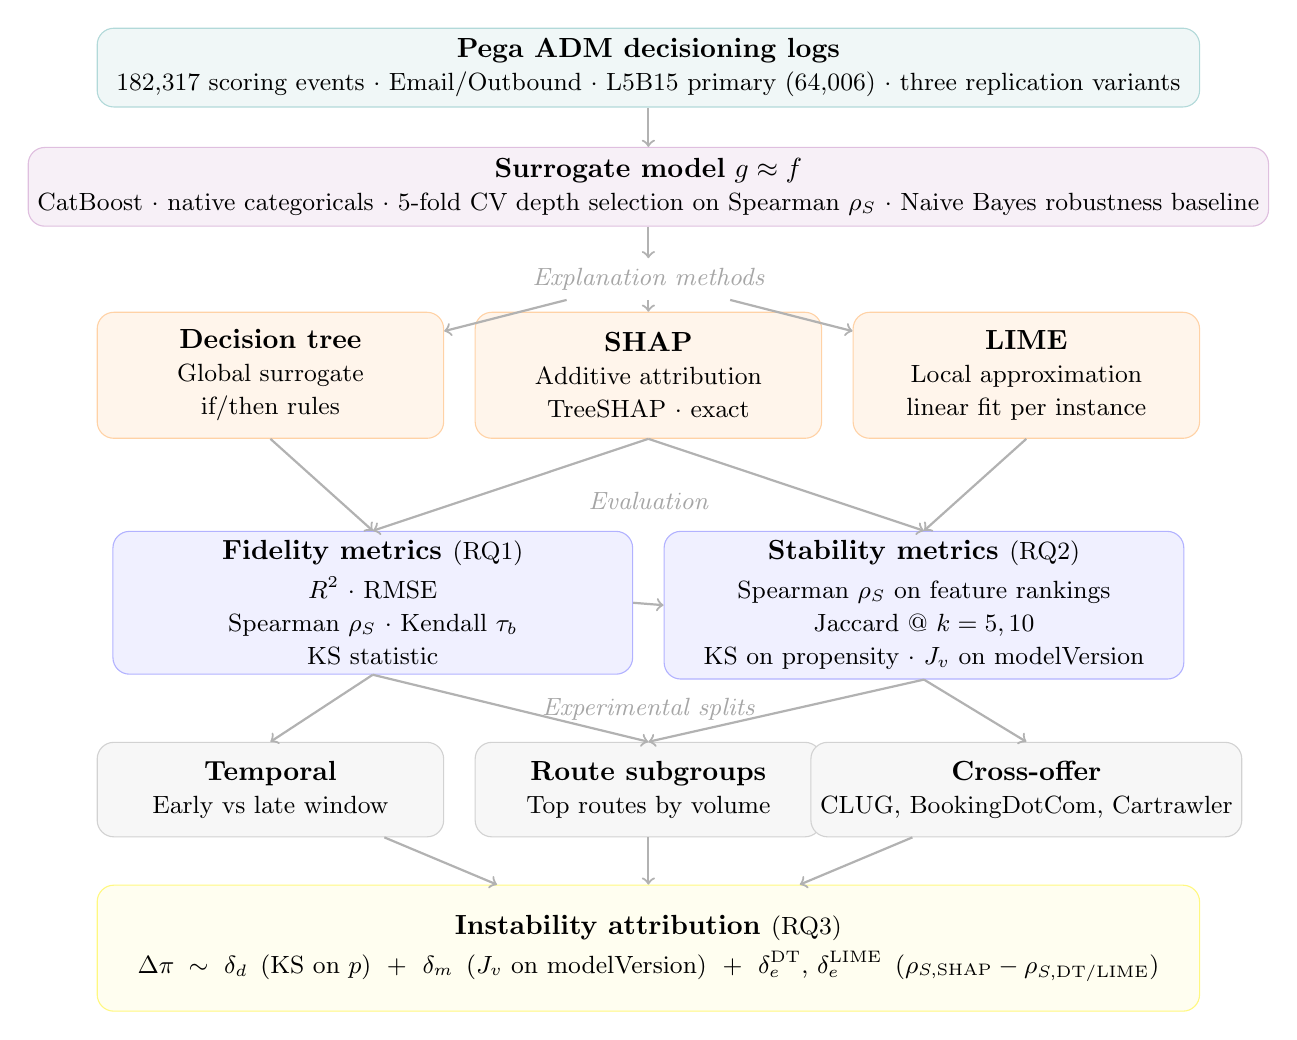
\begin{tikzpicture}[
node distance=0.5cm, box/.style={rectangle, draw, rounded corners=6pt, minimum width=14cm, minimum height=1cm, align=center, fill=gray!8, draw=gray!40}, boxblue/.style={rectangle, draw, rounded corners=6pt, minimum width=6.6cm, minimum height=1.8cm, align=center, fill=blue!6, draw=blue!30}, boxcoral/.style={rectangle, draw, rounded corners=6pt, minimum width=4.4cm, minimum height=1.6cm, align=center, fill=orange!8, draw=orange!35}, boxgray/.style={rectangle, draw, rounded corners=6pt, minimum width=4.4cm, minimum height=1.2cm, align=center, fill=gray!6, draw=gray!35}, boxamber/.style={rectangle, draw, rounded corners=6pt, minimum width=14cm, minimum height=1.6cm, align=center, fill=yellow!6, draw=yellow!50}, boxteal/.style={rectangle, draw, rounded corners=6pt, minimum width=14cm, minimum height=1cm, align=center, fill=teal!6, draw=teal!30}, boxpurple/.style={rectangle, draw, rounded corners=6pt, minimum width=14cm, minimum height=1cm, align=center, fill=violet!6, draw=violet!25}, arrow/.style={->, thick, gray!60}, label/.style={font=\small\itshape, text=gray!70} ]
\node[boxteal] (data) {\textbf{Pega ADM decisioning logs}\\{\small 182,317 scoring events $\cdot$ Email/Outbound $\cdot$ L5B15 primary (64,006) $\cdot$ three replication variants}};
\node[boxpurple, below=of data] (surrogate) {\textbf{Surrogate model} $g \approx f$\\{\small CatBoost $\cdot$ native categoricals $\cdot$ 5-fold CV depth selection on Spearman $\rho_S$ $\cdot$ Naive Bayes robustness baseline}};
\node[label, below=0.4cm of surrogate] (xailabel) {Explanation methods};
\node[boxcoral, below=0.15cm of xailabel, xshift=-4.8cm] (dt) {\textbf{Decision tree}\\{\small Global surrogate}\\{\small if/then rules}};
\node[boxcoral, below=0.15cm of xailabel] (shap) {\textbf{SHAP}\\{\small Additive attribution}\\{\small TreeSHAP $\cdot$ exact}};
\node[boxcoral, below=0.15cm of xailabel, xshift=4.8cm] (lime) {\textbf{LIME}\\{\small Local approximation}\\{\small linear fit per instance}};
\node[label, below=0.55cm of shap] (evallabel) {Evaluation};
\node[boxblue, below=0.15cm of evallabel, xshift=-3.5cm] (fidelity) {\textbf{Fidelity metrics \normalfont\small(RQ1)}\\[2pt]{\small $R^2$ $\cdot$ RMSE}\\{\small Spearman $\rho_S$ $\cdot$ Kendall $\tau_b$}\\{\small KS statistic}};
\node[boxblue, below=0.15cm of evallabel, xshift=3.5cm] (stability) {\textbf{Stability metrics \normalfont\small(RQ2)}\\[2pt]{\small Spearman $\rho_S$ on feature rankings}\\{\small Jaccard @ $k = 5, 10$}\\{\small KS on propensity $\cdot$ $J_v$ on modelVersion}};
\node[label, below=0.55cm of evallabel, yshift=-1.6cm] (splitlabel) {Experimental splits};
\node[boxgray, below=0.15cm of splitlabel, xshift=-4.8cm] (temporal) {\textbf{Temporal}\\{\small Early vs late window}};
\node[boxgray, below=0.15cm of splitlabel] (route) {\textbf{Route subgroups}\\{\small Top routes by volume}};
\node[boxgray, below=0.15cm of splitlabel, xshift=4.8cm] (crossoffer) {\textbf{Cross-offer}\\{\small CLUG, BookingDotCom, Cartrawler}};
\node[boxamber, below=0.6cm of route] (instability) {\textbf{Instability attribution \normalfont\small(RQ3)}\\[2pt]{\small $\Delta\pi \;\sim\;$ $\delta_d$ \,(KS on $p$) $\;+\;$ $\delta_m$ \,($J_v$ on modelVersion) $\;+\;$ $\delta_e^{\mathrm{DT}}$, $\delta_e^{\mathrm{LIME}}$ \,($\rho_{S,\mathrm{SHAP}}-\rho_{S,\mathrm{DT/LIME}}$)}};
\draw[arrow] (data) -- (surrogate);
\draw[arrow] (surrogate) -- (xailabel);
\draw[arrow] (xailabel) -- (dt);
\draw[arrow] (xailabel) -- (shap);
\draw[arrow] (xailabel) -- (lime);
\draw[arrow] (dt.south) -- (fidelity.north);
\draw[arrow] (shap.south) -- (fidelity.north);
\draw[arrow] (shap.south) -- (stability.north);
\draw[arrow] (lime.south) -- (stability.north);
\draw[arrow] (fidelity.east) -- (stability.west);
\draw[arrow] (fidelity.south) -- (temporal.north);
\draw[arrow] (fidelity.south) -- (route.north);
\draw[arrow] (stability.south) -- (route.north);
\draw[arrow] (stability.south) -- (crossoffer.north);
\draw[arrow] (temporal) -- (instability);
\draw[arrow] (route) -- (instability);
\draw[arrow] (crossoffer) -- (instability);
\end{tikzpicture}
\caption{Overview of the methodology. Pega ADM decisioning logs are used to train a
surrogate model $g$, which serves as the prediction oracle for three explanation methods. Each method is evaluated on fidelity against logged propensity scores and stability across experimental splits. Observed instability is decomposed into three sources as the primary methodological contribution.}
\label{fig:methodology_overview}
\end{figure}

\section{Data} \label{sec:data}

The raw data consists of Pega CDH interaction records exported as nested JSON files from a large European passenger airline. Each interaction record contains the full decisioning context for a single customer contact, including all candidate offers evaluated, the selected action, and the propensity scores assigned to each offer. Records are parsed and deduplicated on a unique execution identifier to prevent double-counting across overlapping exports. After filtering to the Email and Outbound channel and retaining only sales actions, the working dataset contains 180,957 scoring events across four offer variants. Minor luggage variants with fewer than 2,000 observations combined are present in the raw data but excluded from analysis due to insufficient volume for stable surrogate training and split-based evaluation.

The 180,957 scoring events span four analysed variants summarised in Table~\ref{tab:variants}. The primary analysis focuses on the 15\,kg luggage add-on variant (L5B15, $n = 64{,}006$), selected as the highest-volume weight-specific offer and the most commercially established product in the portfolio. Three further variants are retained as replication cases: the generic luggage offer (CLUG, $n = 34{,}230$), which shares the same product context as L5B15; and two third-party partner offers, BookingDotCom ($n = 40{,}561$, accommodation) and Cartrawler ($n = 42{,}160$, car rental), which operate in entirely different product categories. Including partner offers alongside luggage variants tests whether explanation behaviour generalises not only across models with similar feature spaces but across models with different commercial contexts, providing a stronger generalisability check for RQ4 than weight-variant replication alone. Each variant is governed by its own independently-updating Pega ADM instance with a partially distinct set of active predictors, so replication is conducted within each variant's own feature space.

\begin{table}[ht]
\caption{Volume by offer variant. Replication variants span both luggage and third-party
partner offer types.}
\label{tab:variants}
\centering
\begin{tabular}{llr}
\toprule
Variant & Type & $n$ \\
\midrule
L5B15 & 15\,kg luggage add-on (primary) & 64,006 \\
CLUG & Generic luggage offer & 34,230 \\
BookingDotCom & Third-party accommodation offer & 40,561 \\
Cartrawler & Third-party car rental offer & 42,160 \\
\bottomrule
\end{tabular}
\end{table}

The feature space is restricted to the predictors confirmed active in the live Pega ADM model for each variant, as identified from ADM model snapshots. This restriction is deliberate: Pega ADM automatically selects and deactivates predictors based on their evidential contribution, disabling those whose association with the target falls below an internal threshold. Including inactive predictors would mean training a surrogate on features the black-box model does not use, causing explanations to reflect the surrogate's own behaviour rather than that of the model being explained. The number of active predictors varies across variants, ranging from 22 in the CLUG variant to 33 in BookingDotCom, reflecting each model's independent predictor selection. Predictors span four feature groups: booking context, flight data, contact history, and scoring parameters, with customer attributes appearing additionally in the BookingDotCom variant only. Missingness varies substantially across groups: flight data features are largely complete across all variants (mean 1.1--2.1\%), while contact history features are considerably sparser (mean 41.6--57.4\%), reflecting customers with limited or no prior contact history on a given channel. Scoring parameters are populated at scoring time rather than read from a customer record, so the parquet column underlying the CatBoost categorical encoding has no row-level absence to count (indicated with a dash in the appendix table). A full breakdown of active predictor counts and missingness by feature group and variant is provided in Appendix~\ref{app:missingness}.

The target variable is the Pega ADM propensity score $p \in [0,1]$, representing the model's estimated purchase probability at the moment of scoring. Observed purchase outcomes are not used as the target: the goal of this study is to explain what drives Pega's model output, not to model customer behaviour directly. Using observed outcomes would require assumptions about exposure and selection that cannot be satisfied with observational decisioning data. A further structural characteristic of the dataset is that the underlying model is not static: Pega ADM updates its Naive Bayes model continuously via online learning, meaning different customers in the observation window were scored by different model snapshots. Each scoring event is logged with a model-version identifier denoting which snapshot produced the propensity score, alongside descriptive metadata on the number of customer responses and the model's AUC at the time. The model-version field is excluded from the surrogate feature matrix but retained as the diagnostic proxy for model version churn in the instability attribution analysis in Section~\ref{sec:evaluation}.

\section{Surrogate Model} \label{sec:surrogate}

Because direct queries to the Pega ADM model $f$ are unavailable, all explanation methods operate through a surrogate model $g$ trained to approximate $f$ on the observed logged scores. The surrogate serves two roles: as the prediction oracle required by SHAP and LIME, and as the first stage of fidelity evaluation, since the quality of any downstream explanation is bounded by how accurately $g$ replicates $f$'s input-output mapping.

Rather than fixing the surrogate architecture on theoretical grounds alone, five candidate models are compared empirically on the L5B15 dataset using the full suite of fidelity metrics defined in Section~\ref{sec:evaluation}, with the final selection based on performance across all five metrics jointly. The candidates represent a range of model complexity and different approaches to handling categorical features: linear regression as a lower bound, Gaussian Naive Bayes as an architecture-matched baseline given that Pega ADM uses Naive Bayes internally, Random Forest and LightGBM as alternative flexible models, and CatBoost as the proposed surrogate. All five candidates are evaluated on the same stratified 80/20 train/test split, stratified on propensity decile bins to ensure the test set covers the full propensity range, which is important for rank-based and distributional metrics. The full comparison is reported at the start of Section~\ref{ch:results}.

Beyond rank-based fidelity, two additional properties guide the final architecture choice. The first is compatibility with TreeSHAP, the SHAP implementation used in this study. TreeSHAP computes exact Shapley values analytically by exploiting the tree structure of the model, which is only possible for tree-based architectures. Applying SHAP to a non-tree surrogate would require KernelSHAP instead, a model-agnostic approximation that introduces its own sampling variance on top of the surrogate approximation error, compounding exactly the sources of inexactness the study aims to isolate. The second property is categorical encoding. Several candidates require ordinal encoding as a preprocessing step, which assigns arbitrary integer values to categorical levels and introduces a numeric ordering that has no real-world meaning. A surrogate that handles categoricals natively avoids this: it learns directly from the categorical values themselves, meaning that SHAP attributions reflect the true categorical relationships driving propensity scores rather than an arbitrary encoding artefact. Missing values in sparse features such as contact history are handled in the same way, preserving absence of information as a meaningful signal consistent with how Pega ADM treats its own missing predictor bins.

Tree depth is treated as a tuning parameter selected independently per variant via five-fold cross-validation on Spearman $\rho_S$ over depths 1 to 15, using 200 boosting iterations during the depth sweep and 500 for the final fit. The reduced iteration budget during cross-validation is sufficient because the relative ranking of depths stabilises well before convergence. Breiman's 1-SD rule is applied to the resulting CV curve
\parencite{hastie_elements_2009}: the selected depth is the smallest value whose mean $\rho_S$
falls within one fold-to-fold standard deviation of the CV maximum, operationalising the principle that when several depths are statistically indistinguishable from the best, the simplest should be preferred. The grid upper bound of 15 is chosen to extend past CatBoost's typical effective depth on tabular data by a sufficient margin to confirm that the mean-$\rho_S$ curve plateaus inside the grid rather than at its edge, which would indicate a range-cap artefact rather than a genuine optimum. Selected depths and final fidelity results per variant are reported in Section~\ref{ch:results}.

\section{Explanation Methods} \label{sec:explanation_methods}

Three post-hoc explanation methods are evaluated, representing fundamentally different approaches to interpreting black-box model predictions: additive feature attribution via SHAP, local linear approximation via LIME, and global rule-based approximation via a shallow decision tree surrogate. All three methods operate on logged propensity scores $p_i = f(\mathbf{X}_i)$ rather than a live scoring API, reflecting the realistic constraint that Pega ADM's internals are inaccessible. SHAP and LIME both require a callable prediction function and therefore use the CatBoost surrogate $g$ as their oracle, inducing the two-layer approximation pipeline $f \rightarrow g \rightarrow \boldsymbol{\phi}$ established in Section~\ref{sec:formulation}. The decision tree surrogate is fitted directly on $p_i$ and does not require an intermediate model, introducing only a single layer of approximation error.

\subsection{Global Surrogate: Decision Tree}

A shallow regression tree is fitted directly on the logged propensity scores $p_i = f(\mathbf{X}_i)$, providing a globally interpretable approximation of the black-box model's input-output mapping. Tree depth is treated as a hyperparameter and selected by five-fold cross-validation optimising Spearman rank correlation over the range one to ten, consistent with the surrogate model depth selection described in Section~\ref{sec:surrogate}. Because the decision tree is implemented via scikit-learn rather than CatBoost, categorical features are encoded using ordinal encoding prior to fitting. This encoding choice is a practical constraint of the sklearn interface rather than a modelling preference; its potential effect on feature importance rankings relative to the CatBoost-based methods is acknowledged as a limitation in Section~\ref{sec:assumptions}. Decision rules are extracted as human-readable if/then conditions, producing a compact summary of the dominant decision logic governing propensity scores across the full dataset. Fidelity is assessed using the metrics defined in Section~\ref{sec:evaluation}.

\subsection{SHAP}

SHAP (SHapley Additive exPlanations) decomposes each prediction into an additive sum of feature contributions grounded in cooperative game theory \parencite{lundberg_unified_2017}. For a prediction $q_i = g(\mathbf{X}_i)$, SHAP assigns each feature $j$ a scalar value $\phi_j(\mathbf{X}_i)$ such that
\[
q_i = \phi_0 + \sum_{j=1}^{d} \phi_j(\mathbf{X}_i),
\]
where $\phi_0 \in \mathbb{R}$ is the expected model output over the training data, $\phi_0 = \mathbb{E}[g(\mathbf{X})]$, and $\boldsymbol{\phi}(\mathbf{X}_i) = (\phi_1(\mathbf{X}_i), \ldots, \phi_d(\mathbf{X}_i))$ is the vector of instance-level attributions introduced in Section~\ref{sec:formulation}. The completeness axiom guarantees that attributions sum exactly to the model output, providing an internally consistent decomposition by construction. SHAP values are computed using TreeSHAP, which exploits the tree structure of the CatBoost surrogate to derive exact Shapley values analytically, avoiding the sampling variance introduced by model-agnostic approximations such as KernelSHAP \parencite{lundberg_unified_2017}. Global feature importance is summarised as mean absolute SHAP values aggregated across all instances. Because SHAP values are computed on $g$ rather than $f$ directly, explanation fidelity inherits from surrogate fidelity, assessed using the metrics defined in Section~\ref{sec:evaluation}.

\subsection{LIME}

LIME (Local Interpretable Model-agnostic Explanations) approximates model behaviour in the neighbourhood of individual predictions using a locally fitted linear model \parencite{ribeiro_why_2016}. For a given instance $\mathbf{X}_i$, LIME generates a set of perturbed samples in the vicinity of $\mathbf{X}_i$, queries the surrogate $g$ to obtain predicted propensity scores for each perturbed sample, and fits a weighted linear regression to the resulting input-output pairs. The linear coefficients serve as local feature importances for that instance. In this study, the CatBoost surrogate serves as the prediction oracle: LIME perturbs instances and queries $g$ rather than Pega's live API, which is consistent with the black-box access constraint and ensures that all explanation methods operate under identical conditions. LIME explanations are computed for a sample of 500 instances with 200 perturbations per instance, balancing computational cost against coverage of the feature space. LIME's perturbation mechanism produces binned condition strings rather than raw feature names; these are mapped back to base feature names before aggregation. Global importance is summarised as mean absolute LIME coefficients across all sampled instances. For SHAP and the decision tree surrogate, importance scores are well-defined globally and aggregation is straightforward. For LIME, this aggregation assumes coefficient comparability across instances, which may not hold in all regions of the feature space and is treated as a limitation in Section~\ref{sec:assumptions}. Local fidelity is measured as the $R^2$ of LIME's linear fit for each individual instance, capturing how well the linear approximation describes $g$'s behaviour in that neighbourhood. Unlike the global fidelity metrics in Section~\ref{sec:formulation}, this is an instance-level quantity reported as a distribution with its mean and standard deviation across all evaluated instances.

\section{Evaluation Framework} \label{sec:evaluation}

Explanation quality is assessed along two dimensions established in Section~\ref{sec:formulation}: fidelity, measuring how accurately each explanation method approximates the black-box propensity scores, and stability, measuring how consistently feature attribution rankings are reproduced across different evaluation splits. This section provides formal definitions of all metrics used to operationalise these dimensions.

\subsection{Fidelity Metrics}

Fidelity is assessed using four complementary metrics, each capturing a different aspect of surrogate agreement with the logged propensity scores $p_i = f(\mathbf{X}_i)$. Let $q_i = g(\mathbf{X}_i)$ denote the surrogate prediction for instance $i$ on a held-out test set of size $n$.

The coefficient of determination is defined as
\[
R^2 = 1 - \frac{\sum_{i=1}^{n}(p_i - q_i)^2}{\sum_{i=1}^{n}(p_i - \bar{p})^2},
\]
where $\bar{p} = \frac{1}{n}\sum_{i=1}^{n} p_i$ is the mean logged propensity score. $R^2$ measures the proportion of variance in $p$ explained by $g$, with values closer to one indicating higher fidelity.

Root mean squared error is defined as
\[
\text{RMSE} = \sqrt{\frac{1}{n}\sum_{i=1}^{n}(p_i - q_i)^2},
\]
providing a pointwise measure of prediction error on the scale of the propensity scores themselves.

Spearman rank correlation $\rho_S$ and Kendall's $\tau_b$ are computed between the vectors $(p_1, \ldots, p_n)$ and $(q_1, \ldots, q_n)$. Both measure rank preservation: whether the surrogate orders instances in the same way as the black-box model. Spearman's $\rho_S$ is defined as the Pearson correlation of the rank-transformed scores:
\[
\rho_S = \frac{\sum_{i=1}^{n}(R_i - \bar{R})(T_i - \bar{T})} {\sqrt{\sum_{i=1}^{n}(R_i - \bar{R})^2 \sum_{i=1}^{n}(T_i - \bar{T})^2}},
\]
where $R_i$ and $T_i$ denote the ranks of $p_i$ and $q_i$ respectively, and $\bar{R}$, $\bar{T}$ are the corresponding mean ranks. Kendall's $\tau_b$ accounts for tied ranks and is defined as
\[
\tau_b = \frac{|\text{concordant pairs}| - |\text{discordant pairs}|} {\sqrt{(C - T_p)(C - T_q)}},
\]
where $C = \binom{n}{2}$ is the total number of pairs, $T_p$ is the number of pairs tied on $p$, and $T_q$ is the number of pairs tied on $q$. Rank preservation is treated as the primary fidelity criterion, as Pega CDH uses propensity scores to rank and prioritise offers rather than as calibrated probabilities, making order-consistency more relevant than pointwise accuracy for downstream decisioning.

Distributional alignment is assessed using the two-sample Kolmogorov-Smirnov statistic:
\[
D_{KS} = \sup_{x} \left| F_p(x) - F_q(x) \right|,
\]
where $F_p$ and $F_q$ are the empirical cumulative distribution functions of the logged and surrogate propensity scores respectively. A small $D_{KS}$ indicates that the surrogate reproduces the overall shape of the propensity score distribution.

\subsection{Stability Metrics}

Stability is defined as the consistency of feature importance rankings across evaluation splits. Let $\pi_t = (\pi_t^{(1)}, \ldots, \pi_t^{(d)})$ denote the ranking of the $d$ active predictors induced by their mean absolute importance score over split $t$, where rank one denotes the most important feature and the specific importance measure is defined by each explanation method. Here $t_1$ and $t_2$ denote the two splits being compared.

Full ranking consistency is measured using Spearman rank correlation between $\pi_{t_1}$ and $\pi_{t_2}$, defined as the Pearson correlation of the rank vectors:
\[
\rho_S(\pi_{t_1}, \pi_{t_2}) =
\frac{\sum_{j=1}^{d}\bigl(\pi_{t_1}^{(j)} - \bar{\pi}_{t_1}\bigr)
\bigl(\pi_{t_2}^{(j)} - \bar{\pi}_{t_2}\bigr)} {\sqrt{\sum_{j=1}^{d}\bigl(\pi_{t_1}^{(j)} - \bar{\pi}_{t_1}\bigr)^2
\sum_{j=1}^{d}\bigl(\pi_{t_2}^{(j)} - \bar{\pi}_{t_2}\bigr)^2}},
\]
where $\bar{\pi}_{t} = \frac{1}{d}\sum_{j=1}^{d}\pi_t^{(j)}$ is the mean rank in split $t$. Values close to one indicate that the full feature ranking is preserved across splits; values close to zero indicate that rankings are essentially uncorrelated.

Top-$k$ overlap is measured using the Jaccard similarity coefficient between the sets of top-$k$ features identified in each split:
\[
J_k(\pi_{t_1}, \pi_{t_2}) = \frac{|S_{t_1}^{(k)} \cap S_{t_2}^{(k)}|}{|S_{t_1}^{(k)} \cup S_{t_2}^{(k)}|},
\]
where $S_t^{(k)}$ denotes the set of the $k$ highest-ranked features in split $t$. Jaccard similarity is evaluated at $k = 5$ and $k = 10$: $k = 5$ captures the features a practitioner would inspect first; $k = 10$ captures broader agreement across the top half of the active predictor set. A value of one indicates perfect overlap; zero indicates no shared features in the top-$k$. Both metrics are computed for each explanation method separately across temporal, route-based, and culture-based splits, and reported as a summary table enabling direct comparison of stability across SHAP, LIME, and the decision tree surrogate.

To validate that observed between-split decision tree instability reflects genuine subgroup sensitivity rather than random fitting variance, a bootstrap procedure is applied: the decision tree is re-fitted ten times on the same data using different random seeds, and the spread in feature rankings is compared against the between-split instability gap. A between-split gap that exceeds the bootstrap variance confirms that instability is attributable to subgroup composition rather than fitting noise.

\subsection{Instability Attribution}

Observed instability $\Delta\pi = 1 - \rho_S(\pi_{t_1}, \pi_{t_2})$ may reflect any combination of three sources introduced in Section~\ref{sec:formulation}: distribution shift $\delta_d$, model version churn $\delta_m$, and explainer sensitivity $\delta_e$. Because all three sources operate simultaneously in observational CDH data, a precise causal decomposition is not possible. Instead, this study proposes a structured diagnostic that jointly characterises each source and uses their co-occurrence pattern to attribute instability to its likely dominant cause. All thresholds are applied to effect-size statistics directly; p-values are intentionally omitted because at sample sizes in the thousands, even trivially small effect sizes reach conventional significance levels.

Distribution shift $\delta_d$ is monitored using the two-sample Kolmogorov-Smirnov statistic on the propensity score distribution across splits. KS was chosen over PSI because Pega ADM maps log-odds scores to propensities via an isotonic calibration step that produces a step function: instances in the same score bin all receive the same propensity value. The resulting distribution clusters on a small set of recurring values rather than spreading continuously across $[0, 1]$, which causes PSI to be sensitive to where bin boundaries fall and to inflate artificially when bins split these clustered values unevenly. KS operates directly on empirical CDFs without any binning or smoothing parameter, making it robust to this artefact. The PSI bin-sensitivity analysis is documented in Appendix~\ref{app:psi_sensitivity} as a transparency check. A propensity distribution shift is classified as significant when $\text{KS}_{\hat{p}} \geq 0.10$, a threshold that corresponds to a maximum ECDF gap of ten percentage points and is consistent with standard drift-detection practice.

Model version churn $\delta_m$ is proxied by the Jaccard overlap between the sets of model snapshot identifiers active in each split:
\[
J_v = \frac{|V_{t_1} \cap V_{t_2}|}{|V_{t_1} \cup V_{t_2}|},
\]
where $V_t$ is the set of distinct model snapshot identifiers observed in split $t$. A value near zero indicates that the two splits were scored by largely non-overlapping snapshots; a value near one indicates substantial overlap. Pega ADM assigns a new snapshot identifier on every micro-update of the online Naive Bayes, so $J_v$ measures snapshot turnover rather than parameter shift directly: two functionally identical models may carry different identifiers if an update occurred between splits. This limitation is mitigated by a structural property of the route and culture splits used in this study. Because those splits are drawn from the same observation window, the production scorer was drawing on the same pool of active snapshots by construction, and any reasonable $\delta_m$ proxy returns a value near zero for those splits. The RQ3 conclusion is therefore robust to the choice of churn proxy, even if $J_v$ alone is imperfect as a general parameter-shift metric. Model version churn is classified as significant when $J_v \leq 0.10$. This threshold sits in an empirically observed gap in the bimodal distribution of $J_v$ values: temporal splits produce values near zero while same-window splits produce values near $0.5$, with no observed values in the interval $(0.10, 0.40)$. A sensitivity analysis varying the threshold across this interval confirms that split classifications are invariant, as documented in Appendix~\ref{app:jaccard_sensitivity}.

Explainer sensitivity $\delta_e$ captures how much of the observed ranking instability stems from the explanation method itself, rather than from changes in the data or the model. SHAP serves as the reference because TreeSHAP is deterministic given a fixed surrogate: a single CatBoost surrogate is fitted once on the full training set and applied identically to both splits, so any change in SHAP rankings reflects only $\delta_d$ and $\delta_m$ with no contribution from refitting or sampling variance. The decision tree and LIME explainers are then compared against this reference, probing two distinct mechanisms of explainer sensitivity:
\begin{itemize}
\item DT refit sensitivity, $\delta_e^{\text{DT}} \approx \rho_{S,\text{SHAP}} - \rho_{S,\text{DT}}$, captures variance from re-fitting the surrogate tree structure independently on each split.
\item LIME sampling sensitivity, $\delta_e^{\text{LIME}} \approx \rho_{S,\text{SHAP}} - \rho_{S,\text{LIME}}$, captures variance from LIME's local perturbation sampling. LIME shares the fixed-surrogate property with SHAP, so any gap here is sampling-side, not refit-side.
\end{itemize}
A positive value indicates that the corresponding explainer is less stable than SHAP beyond what $\delta_d$ and $\delta_m$ alone would predict. The two diagnostics are complementary of the same instability construct and are reported jointly throughout the Results.

The three diagnostic measures are combined into a classification rule summarised in Table~\ref{tab:attribution_rule}. Each split is assigned to its primary instability source based on the co-occurrence of the two external-source diagnostics, $\text{KS}_{\hat{p}}$ and $J_v$. The explainer gaps $\delta_e^{\text{DT}}$ and $\delta_e^{\text{LIME}}$ are reported alongside the classification as descriptive evidence; they are not classifier inputs, but they validate an Explainer assignment when large and qualify a Distribution shift, Model churn, or Both assignment when small.

\begin{table}[ht]
\caption{Attribution classification rule. Each split is assigned to its primary instability source based on the two external-source diagnostics. $\text{KS}_{\hat{p}}$ threshold $\geq 0.10$; $J_v$ threshold $\leq 0.10$. The explainer-sensitivity gaps $\delta_e^{\text{DT}}$ and $\delta_e^{\text{LIME}}$ are reported as descriptive evidence, not thresholded.}
\label{tab:attribution_rule}
\centering
\begin{tabular}{lccp{6cm}}
\toprule
Primary source & $\text{KS}_{\hat{p}} \geq 0.10$ & $J_v \leq 0.10$ & Interpretation \\
\midrule
Explainer ($\delta_e$) & No & No & External conditions stable; residual instability attributed to the explanation method (refitting or sampling variance) \\
Dist.\ shift ($\delta_d$) & Yes & No & Propensity distribution shifted across splits; input data or upstream pipeline changed \\
Model churn ($\delta_m$) & No & Yes & Model snapshot turnover significant; underlying model updated between splits \\
Both ($\delta_d + \delta_m$) & Yes & Yes & Both external conditions triggered simultaneously \\
\bottomrule
\end{tabular}
\end{table}

This pattern-based attribution does not claim causal precision but provides a principled and transparent basis for interpreting explanation instability in production CDH environments.

\section{Experimental Design} \label{sec:experimental_design}

Evaluation splits are constructed across four dimensions. Temporal splits divide each variant's observation window into an early and late period at the median decision timestamp, ensuring roughly equal sample sizes in each half. Route subgroups are constructed from the three highest-volume departure-destination pairs in L5B15. As shown in Table~\ref{tab:route_pairs}, the three adjacent pairs are structured to cover shared origin, shared destination, and no shared element, providing a systematic basis for assessing whether origin or destination drives explanation instability.

\begin{table}[ht]
\caption{Route subgroup pairs for L5B15 stability evaluation, constructed from the four 
highest-volume routes.}
\label{tab:route_pairs}
\centering
\begin{tabular}{llll}
\toprule
Pair & Route A & Route B & Comparison type \\
\midrule
1 & ORY$\to$NCE & ORY$\to$OPO & Shared origin, different destination \\
2 & ORY$\to$OPO & NCE$\to$ORY & Different origin, different destination \\
3 & NCE$\to$ORY & TLS$\to$ORY & Different origin, shared destination \\
\bottomrule
\end{tabular}
\end{table}

Culture subgroups compare the two highest-volume customer culture codes in L5B15, French (FR) and Dutch (NL), providing a customer-segment dimension alongside the route-based splits. The same temporal split is applied to the three replication variants (CLUG, BookingDotCom, and Cartrawler) to test whether the stability and attribution patterns found for L5B15 generalise to offer models with different product contexts and partially distinct feature sets.

\section{Feature-Driver Analysis} \label{sec:rq5_method}

RQ1--RQ4 evaluate the explanation methods themselves: whether SHAP, LIME, and the decision-tree surrogate reproduce the Pega scores faithfully (RQ1), whether their feature rankings are stable across temporal, route, and culture splits (RQ2), how observed shifts decompose across distribution, model-churn, and explainer sources (RQ3), and whether the picture replicates across offer variants (RQ4). Those four questions deliver the licence RQ5 requires: when the three methods agree that a feature carries high importance under the fidelities and stabilities documented in earlier chapters, the ranking can be read as the production model's own signal rather than an explainer artefact. RQ5 therefore proceeds to the content-level question, namely which features the production model has in fact learned to score on. The analysis is purely associative and makes no causal claim about which features cause add-on uptake; it characterises only the importance the production model attributes to them. It introduces no new model and re-uses the per-feature importances produced by SHAP, LIME, and the surrogate decision tree on L5B15.

The procedure has three steps. First, each method's importances are normalised to sum to one and ranked, yielding a cross-method view of which individual predictors carry the most weight. Predictors are then assigned to one of four feature groups, contact history, flight data, booking context, and scoring parameter, using the same grouping as the importance heatmap (Figure~\ref{fig:feature_importance_heatmap}), and importance is summed within group to give each group's share of total attribution per method. The group-level view is the primary summary, motivated directly by RQ2--RQ3: even where individual ranks shift modestly across splits, group-level shares are far less sensitive, because the within-group reshuffling of importance across correlated predictors, which RQ3 partly attributes to explainer sensitivity $\delta_e$, cancels under aggregation. Group shares therefore inherit the stability evidence of RQ2 more cleanly than individual ranks do.

Second, for each predictor in the upper portion of the cross-method ranking, we ask whether a business-logical link to luggage add-on uptake is present. Recency and frequency of prior outbound contact pass this check as a contact-fatigue proxy, trip-context fields such as seat number, destination, or booking month as a trip-type or party-size proxy, and the scoring parameter because it encodes which offer is being scored. A predictor fails the check if no such link is available on its face. This step is judgmental rather than statistical and is reported transparently; its role is not to validate the model but to surface predictors whose attributed importance demands a follow-up before reaching a stakeholder.

Third, a flagged predictor is probed in the raw data to establish whether the surrogate's importance attribution tracks the field's \emph{value} or its mere \emph{populated-ness}. The latter mechanism is plausible in this setting because Pega ADM's predictor selection groups predictors with pairwise correlation above an internal threshold and retains only the strongest of each group; a single surviving predictor can therefore silently encode the missingness pattern of an entire dropped cluster. The probe returns to the full pre-restriction feature matrix (441 columns, 64{,}006 L5B15 records) and constructs three variables. Let $Z = \mathbf{1}[\text{predictor populated}]$ denote the binary populated-indicator for the flagged predictor (chosen to avoid conflict with the feature-vector $\mathbf{X}$ used elsewhere in the methodology), let
\[
C \;=\; \frac{1}{K}\sum_{k=1}^{K} \mathbf{1}[\text{customer field } k \text{ populated}] \;\in\; [0, 1]
\]
denote a continuous customer-completeness index, where the sum runs over the $K$ logged customer-attribute fields outside the previous-flight family. Let $Y = \mathbf{1}[\text{previous-flight customer profile present}]$ be a binary indicator for the dropped customer family most strongly suspected of being proxied, defined over the previous-flight customer-attribute fields. By construction $C$ and $Y$ are computed from disjoint field sets, so that $r_{pb}(Z, C)$ and $V(Z, Y)$ probe independent slices of the customer namespace. Each of the three measures that follow relates $Z$ to either $Y$ (the risk ratio and Cram\'er's $V$) or $C$ (the point-biserial correlation).

The risk ratio
\[
\mathrm{RR} \;=\; \frac{P(Y = 1 \mid Z = 1)}{P(Y = 1 \mid Z = 0)}
\]
is the stakeholder-readable lift in the probability of carrying a previous-flight profile between the two subpopulations defined by $Z$. It is the most direct single number but speaks only to the dropped family encoded in $Y$. $\mathrm{RR}$ ranges over $[0, \infty)$ with $\mathrm{RR} = 1$ as the null of no association; values above one indicate that $Y$ is more likely when $Z = 1$ and read directly as a fold-change ($\mathrm{RR} = 2$ is a two-fold lift, $\mathrm{RR} = 6$ a six-fold lift), while values below one would indicate the opposite direction and are not expected under the missingness-proxy hypothesis.

The point-biserial correlation between $Z$ and the customer-completeness index $C$,
\[
r_{pb} \;=\; \frac{M_1 - M_0}{s_C} \sqrt{\frac{n_1 \, n_0}{n^{2}}},
\]
where $M_1$ and $M_0$ are the means of $C$ in the $Z = 1$ and $Z = 0$ subgroups, $s_C$ is the standard deviation of $C$, and $n_1$, $n_0$, $n$ are the subgroup and total sample sizes, is the Pearson coefficient adapted to one binary and one continuous variable. It asks whether the flagged predictor's populated-ness co-varies with the average populated-ness of the $K$ other customer-attribute fields summarised in $C$, widening the test from the single dropped family $Y$ to the customer-feature space as a whole. $r_{pb}$ shares the $[-1, 1]$ range of the ordinary Pearson correlation, with $r_{pb} = 0$ the null of no linear association; positive values indicate that the $Z = 1$ subgroup carries higher mean completeness across the other customer fields, negative values the reverse. Cohen's conventions for $r$ provide a rough magnitude scale: $|r_{pb}| \approx 0.1$ small, $0.3$ medium, $0.5$ large.

Cram\'er's $V$ on the $2 \times 2$ contingency between $Z$ and $Y$,
\[
V \;=\; \sqrt{\frac{\chi^{2}}{n}}, \qquad \chi^{2} \;=\; \sum_{i,j} \frac{(O_{ij} - E_{ij})^{2}}{E_{ij}},
\]
with $O_{ij}$ and $E_{ij}$ the observed and expected cell counts under independence (the general Cram\'er denominator $n \cdot \min(r{-}1,\, c{-}1)$ reduces to $n$ for a $2 \times 2$ table), normalises $\chi^{2}$ to $[0, 1]$ so the diagnostic is effectively sample-size invariant. This matters because at $n = 64{,}006$ the raw $\chi^{2}$ statistic and its $p$-value are uninformative: any non-zero association is significant by construction, so effect size, rather than significance, is the diagnostic. $V$ also rests on different distributional assumptions from $\mathrm{RR}$ and $r_{pb}$, so that agreement across all three guards against a finding being an artefact of any single measure. $V$ is bounded in $[0, 1]$ with $V = 0$ the null of statistical independence and $V = 1$ a perfect deterministic relationship; for a $2 \times 2$ table it coincides with the absolute value of the phi coefficient, and the same Cohen-style thresholds apply ($V \approx 0.1$ small, $0.3$ medium, $0.5$ large).

The three measures discriminate between three candidate explanations for a flagged predictor's high attribution, summarised in Table~\ref{tab:rq5_probe_pattern}. A value-driven signal leaves $Z$ unrelated to either $C$ or $Y$, so all three measures sit near their null. A narrow artefact tied to one dropped field couples $Z$ tightly to $Y$ but only weakly to the broader pattern in $C$, so only $\mathrm{RR}$ moves materially. A broad missingness proxy for the dropped customer cluster couples $Z$ to both $Y$ and $C$, elevating all three measures together. The probe is therefore not a single hypothesis test but a small profile of effect sizes, read jointly against the predictor's business-logical story from the second step.

\begin{table}[ht]
\caption{Expected effect-size pattern under each candidate explanation for a flagged predictor's high attribution. The three measures are read jointly; the joint pattern, not any single value, identifies the underlying mechanism.}
\label{tab:rq5_probe_pattern}
\centering
\begin{tabular}{lccc}
\toprule
Candidate explanation & $\mathrm{RR}$ & $r_{pb}$ & $V$ \\
\midrule
Value-driven signal & $\approx 1$ & $\approx 0$ & $\approx 0$ \\
Narrow one-field missingness proxy & $\gg 1$ & $\approx 0$ & small \\
Broad missingness proxy (dropped cluster) & $\gg 1$ & substantial & substantial \\
\bottomrule
\end{tabular}
\end{table}

This probe is offered as a generalisable auditing step for CDH-XAI pipelines, complementing the RQ1 fidelity check: where RQ1 establishes that the explanations are faithful to the surrogate, the probe checks that the surrogate's attribution to a flagged predictor in turn tracks its value rather than the missingness signature of the platform's predictor-selection mechanism. The Pega ADM selection mechanism itself is treated as documented platform behaviour and is not re-derived here.

\section{Assumptions and Limitations} \label{sec:assumptions}

This section documents the assumptions underlying the methodological design and the limitations that constrain the interpretation of results.

The most fundamental assumption is that the CatBoost surrogate $g$ provides a sufficiently faithful approximation of the black-box model $f$ to serve as a valid explanation target. As established in Section~\ref{sec:formulation}, two out of three explanation methods operate on $g$ rather than $f$ directly, meaning that explanation validity is bounded by surrogate fidelity. If $g$ fails to replicate $f$'s input-output mapping in regions of the feature space that matter for attribution, the resulting explanations may misrepresent the black-box model's behaviour regardless of the explanation method applied. This assumption is empirically tested rather than taken for granted: surrogate fidelity is assessed using the full metric suite defined in Section~\ref{sec:evaluation}, and results are interpreted conditional on the fidelity diagnostics reported alongside them.

The decision tree surrogate uses ordinal encoding for categorical features due to scikit-learn compatibility constraints, whereas the CatBoost surrogate uses native ordered target encoding. This encoding difference means that the decision tree and CatBoost surrogates treat categorical features differently, and observed stability differences between the decision tree and SHAP may partly reflect encoding sensitivity rather than purely explainer sensitivity. This is acknowledged as a confound in the $\delta_e$ estimation.

The three-way instability attribution framework decomposes observed explanation instability into distribution shift $\delta_d$, model version churn $\delta_m$, and explainer sensitivity $\delta_e$. This decomposition is a structured approximation rather than a causal identification: the three sources are proxied using the Kolmogorov--Smirnov statistic on propensity and Jaccard overlap on the model version sets, and cannot be fully extracted with observational data. In particular, $\delta_d$ and $\delta_m$ are likely correlated, as continuous model updating is itself driven by incoming response data that also shifts the feature distribution. The attribution diagnostic should therefore be interpreted as an indicative decomposition rather than a precise causal accounting. Additionally, $\delta_m$ proxies snapshot turnover rather than parameter shift directly: Pega ADM issues a fresh model version ID on every micro-update of the online Naive Bayes, so two functionally identical models can carry different identifiers. This limitation is mitigated by the structural property of the route and culture splits: because those splits are drawn from the same observation window, the production scorer draws on the same active snapshot pool by construction, and any reasonable churn proxy returns a value near zero for those splits.

LIME importance rankings are derived by aggregating per-instance linear coefficients across splits. Because each local linear model is fitted independently, coefficients are not guaranteed to be on a comparable scale across instances, which may inflate or deflate apparent stability for LIME relative to SHAP and the decision tree surrogate.

Finally, this study is conducted within a single airline's Email and Outbound channel over a single observation window. Generalisability beyond this setting cannot be assumed. Cross-offer replication across three variants with different product contexts provides a broader internal check than single-offer studies, but does not constitute cross-industry or cross-domain validation. The findings are best interpreted as evidence about XAI method behaviour under the specific conditions of a production CDH environment, with implications for practitioners operating in similar settings.

\chapter{Results} \label{ch:results}
\section{Surrogate Fidelity (RQ1)} \label{sec:rq1}

RQ1 asks how accurately the CatBoost surrogate $g$ approximates the Pega ADM black-box model $f$ on the L5B15 variant. This section reports the candidate model comparison that motivates the architecture choice, the depth selection outcome, and the final fidelity of the selected surrogate against the five metrics defined in Section~\ref{sec:evaluation}.

\subsection{Candidate Model Comparison}

Table~\ref{tab:surrogate_comparison} reports fidelity on the held-out 20\% test set for all five candidate surrogates, evaluated jointly across the full metric suite.

\begin{table}[ht]
\caption{Surrogate architecture comparison on the L5B15 held-out test set (stratified 80/20 split). Five candidates are evaluated on rank-based fidelity (Spearman~$\rho$, Kendall~$\tau$), pointwise accuracy ($R^2$, RMSE), and distributional alignment (KS statistic). Best value per metric in bold.}
\label{tab:surrogate_comparison}
\centering
\begin{tabular}{lrrrrr}
\toprule
Model & $R^2$ & RMSE & Spearman $\rho$ & Kendall $\tau$ & KS statistic \\
\midrule
Linear regression & 0.469 & 0.0070 & 0.736 & 0.534 & 0.221 \\
Naive Bayes & 0.368 & 0.0077 & 0.862 & 0.658 & 0.268 \\
Random Forest & 0.761 & 0.0047 & \textbf{0.934} & 0.788 & 0.139 \\
LightGBM & 0.838 & 0.0039 & 0.924 & 0.779 & \textbf{0.090} \\
CatBoost & \textbf{0.927} & \textbf{0.0026} & 0.933 & \textbf{0.798} & 0.154 \\
\bottomrule
\end{tabular}
\end{table}


CatBoost leads convincingly on the pointwise metrics $R^2$ and RMSE, and on Kendall's~$\tau$, with Random Forest the closest competitor on Spearman~$\rho$ and LightGBM producing the lowest KS statistic. The margins on those two metrics are small, however, while CatBoost's advantages on $R^2$ and RMSE are substantial across all tree-based candidates. The Gaussian Naive Bayes baseline is included as an architecture-matched reference, since the black-box model itself is a Naive Bayes classifier. It outperforms linear regression on rank-based metrics, but lags behind all tree-based candidates across the board. Two further considerations support the CatBoost selection beyond raw performance. First, its native categorical handling avoids the artificial ordering effects introduced by integer-based categorical encodings used in the other tree-based candidates. Second, its tree structure enables exact Shapley value computation via TreeSHAP, as described in Section~\ref{sec:surrogate}. On the full metric suite, CatBoost is therefore the preferred surrogate architecture.

\subsection{Depth Selection}

Five-fold cross-validation over depths 1 to 15 is reported in Appendix~\ref{app:cv_depth}. The CV-maximum is reached at depth 12 and Breiman's 1-SD rule selects depth 10, whose mean $\rho_S$ falls within one standard deviation of the CV maximum. The $\bar{\rho}_S$ curve plateaus across depths 10 to 13 before declining marginally at depths 14 and 15, confirming that the optimum lies well inside the grid and that the 1-SD selection is not an artefact of the search range.

\subsection{Final Surrogate Fidelity}

The CatBoost surrogate fitted at depth 10 on 80\% of the L5B15 data achieves the fidelity reported in Table~\ref{tab:surrogate_comparison} on the held-out 20\%. Across the primary rank-based criteria the surrogate reproduces the ordering of Pega's propensity scores with high fidelity, with $\tau_b$ confirming this concordance at the level of individual pairs. The pointwise fit is similarly strong, with $R^2$ indicating that the surrogate explains the large majority of variance in logged propensity scores. The moderate $D_{KS}$ indicates that the surrogate captures the rank structure of $f$ more faithfully than its absolute score distribution, which is an expected consequence of optimising depth selection on $\rho_S$ rather than a distributional criterion and is acceptable given that rank order is the operationally relevant property of Pega's scoring. Together these results indicate that $g$ provides a sufficiently faithful approximation of $f$ to serve as a valid explanation target, satisfying the core modelling assumption established in Section~\ref{sec:formulation}.

\section{Explanation Stability (RQ2)} \label{sec:rq2}

RQ2 asks how consistently feature importance rankings are reproduced across temporal, route-based, and culture-based splits for the L5B15 variant. Stability is assessed using Spearman rank correlation $\rho_S$ on the full feature ranking and Jaccard similarity at $k = 5$ and $k = 10$, as defined in Section~\ref{sec:evaluation}. Results are reported for all three explanation methods across all five split comparisons in Table~\ref{tab:stability_l5b15}.

\begin{table}[ht]
\caption{Stability of feature importance rankings across L5B15 splits. $\rho_S$ measures full-ranking consistency; $J_5$ and $J_{10}$ measure top-$k$ overlap. Route pair numbering follows Table~\ref{tab:route_pairs}.}
\label{tab:stability_l5b15}
\centering
\begin{tabular}{l rrr rrr rrr}
\toprule
 & \multicolumn{3}{c}{SHAP} & \multicolumn{3}{c}{LIME} & \multicolumn{3}{c}{Decision Tree} \\
\cmidrule(lr){2-4} \cmidrule(lr){5-7} \cmidrule(lr){8-10}
Split & $\rho_S$ & $J_5$ & $J_{10}$ & $\rho_S$ & $J_5$ & $J_{10}$ & $\rho_S$ & $J_5$ & $J_{10}$ \\
\midrule
Temporal & 0.996 & 1.000 & 1.000 & 0.989 & 1.000 & 0.818 & 0.855 & 0.667 & 0.667 \\
Route pair 1 & 0.994 & 1.000 & 1.000 & 0.986 & 0.667 & 0.818 & 0.510 & 0.429 & 0.538 \\
Route pair 2 & 0.990 & 1.000 & 0.818 & 0.858 & 1.000 & 0.818 & 0.584 & 0.250 & 0.667 \\
Route pair 3 & 0.987 & 0.667 & 0.818 & 0.992 & 1.000 & 1.000 & 0.817 & 0.667 & 0.667 \\
Culture (FR / NL) & 0.958 & 0.667 & 1.000 & 0.949 & 1.000 & 0.667 & 0.666 & 0.429 & 0.667 \\
\bottomrule
\end{tabular}
\end{table}


\subsection{SHAP Stability}

SHAP produces the most stable rankings across all splits, with $\rho_S$ ranging from 0.958 to 0.996 and full top-5 overlap on the temporal split and the route pairs. The culture split shows the largest deviation for SHAP, with $J_5 = 0.667$ indicating one feature difference in the top five between FR and NL, though the full-ranking correlation remains high. This high stability is structurally expected: SHAP values are computed from a single surrogate fitted once on the full training set, meaning any variation in rankings across splits reflects only genuine differences in how the surrogate weights features in different subpopulations, with no contribution from method refitting variance.

\subsection{LIME Stability}
LIME rankings are similarly stable across temporal and route splits, with $\rho_S$ exceeding 0.986 in all cases except route pair 2 (ORY$\to$OPO vs NCE$\to$ORY), where $\rho_S$ drops to 0.858. This is the only comparison with no shared origin or destination (Table~\ref{tab:route_pairs}), suggesting that LIME's local linear approximations are more sensitive to subgroup composition when the two groups share no structural route element. The culture split also shows reduced LIME stability relative to other splits, with $J_{10} = 0.667$ indicating three features differ in the top ten between the French and Dutch segments. Despite these cases, LIME's full-ranking stability is substantially higher than the decision tree across every split.

\subsection{Decision Tree Stability}

The decision tree is considerably less stable than SHAP and LIME across all split types. On route splits the instability is most pronounced: $\rho_S$ reaches a minimum of 0.510 for route pair 1 (shared origin, different destination) and 0.584 for route pair 2 (no shared element), with $J_5$ as low as 0.250, indicating that only one of the five top-ranked features is shared between the two routes in that comparison. Route pair 3 (different origin, shared destination) is comparatively more stable at $\rho_S = 0.817$. The culture split produces the second largest instability, with $\rho_S = 0.667$ and $J_5 = 0.429$ indicating that the French and Dutch segments created substantially different decision tree structures. The temporal split is the most stable of the decision tree comparisons at $\rho_S = 0.855$, reflecting that the overall feature distribution shifts only moderately between the early and late observation windows.

To confirm that the observed decision tree instability reflects genuine subgroup sensitivity rather than random fitting variance, a bootstrap procedure is applied as described in Section~\ref{sec:evaluation}: the decision tree is re-fitted ten times on the same data using different random seeds, and the mean pairwise $\rho_S$ across seeds serves as a within-split baseline. Table~\ref{tab:bootstrap_dt_main} reports the results per split. For the temporal and culture comparisons the between-split $\rho_S$ falls clearly below the within-split bootstrap mean, confirming that the observed instability exceeds what fitting noise alone would produce. The culture split shows the largest gap, indicating that the French and Dutch segments produce genuinely different tree structures rather than random variation across fits.

For the route pairs the results are more nuanced. Route pairs 1 and 2 show substantial gaps between the bootstrap baseline and the between-split $\rho_S$, confirming genuine subgroup-driven instability. Route pair 3, however, shows a negative gap: the between-split $\rho_S$ (0.817) slightly exceeds the mean within-split $\rho_S$ (0.802), meaning the observed variation between NCE$\to$ORY and TLS$\to$ORY is fully within the range of normal fitting noise. The decision tree is not meaningfully unstable across this pair. This result contextualises the stability metric in Table~\ref{tab:stability_l5b15}: while $\rho_S = 0.817$ is lower than SHAP or LIME on the same pair, it does not reflect a genuine subgroup difference and should not be interpreted as evidence of explanation instability.

\begin{table}[ht]
\caption{Bootstrap validation of decision tree instability. Within-split $\rho_S$ is the mean pairwise Spearman correlation across ten re-fits on the same data; between-split $\rho_S$ is the observed stability metric from Table~\ref{tab:stability_l5b15}. A positive gap confirms that between-split instability exceeds what fitting noise alone can explain; a negative or near-zero gap indicates that the observed variation falls within the range of random fitting variance.}
\label{tab:bootstrap_dt_main}
\centering
\begin{tabular}{lrrr}
\toprule
Split & Within-split $\rho_S$ & Between-split $\rho_S$ & Gap \\
\midrule
Temporal& 0.935 & 0.855 & 0.080 \\
Route pair 1 (ORY$\to$NCE vs ORY$\to$OPO) & 0.824 & 0.510 & 0.314 \\
Route pair 2 (ORY$\to$OPO vs NCE$\to$ORY) & 0.789 & 0.584 & 0.206 \\
Route pair 3 (NCE$\to$ORY vs TLS$\to$ORY) & 0.802 & 0.817 & $-$0.015 \\
Culture (FR / NL) & 0.977 & 0.667 & 0.310 \\
\bottomrule
\end{tabular}
\end{table}

\subsection{Feature Attribution Content}

Figure~\ref{fig:feature_importance_heatmap} shows the normalised feature importance scores across all splits for each explanation method, with features ordered by mean importance across all splits and methods combined. The SHAP and LIME panels present a smooth, consistent colour gradient across splits: the same features dominate the top rows uniformly, with importance decaying gradually down the ranking and the pattern shifting only marginally between splits. The decision tree panel presents a different picture: high-contrast patches appear in different rows across splits, reflecting the tree's tendency to concentrate importance on whichever single feature is most discriminative in a given subgroup rather than distributing it across the full feature set. This pattern is consistent with the instability gap reported in Table~\ref{tab:stability_l5b15}.

Two levels of stability emerge from this analysis, and the distinction matters for everything that follows. At the level of individual feature ranks, the methods diverge: SHAP and LIME are nearly invariant across splits, the decision tree is materially less stable, and the three methods only partially agree on the precise order of features within the top of the ranking. At the level of feature \emph{groups}, by contrast, all three methods converge on the same broad attribution structure across every split tested. The top-ranked features belong consistently to two feature groups across all splits and methods, contact history features capturing the recency and frequency of prior outbound communications and offer-level scoring parameters, with booking context features playing a secondary but stable role; the decision tree's within-group reshuffling does not propagate to those group-level shares. This second result is the load-bearing finding for any downstream content analysis: irrespective of which method one reads or which split one looks at, the L5B15 explanations are stable enough at the group level to support a substantive reading of which feature groups the production model scores on, which is the question §\ref{sec:rq5} takes up.

\begin{figure}[ht]
\centering
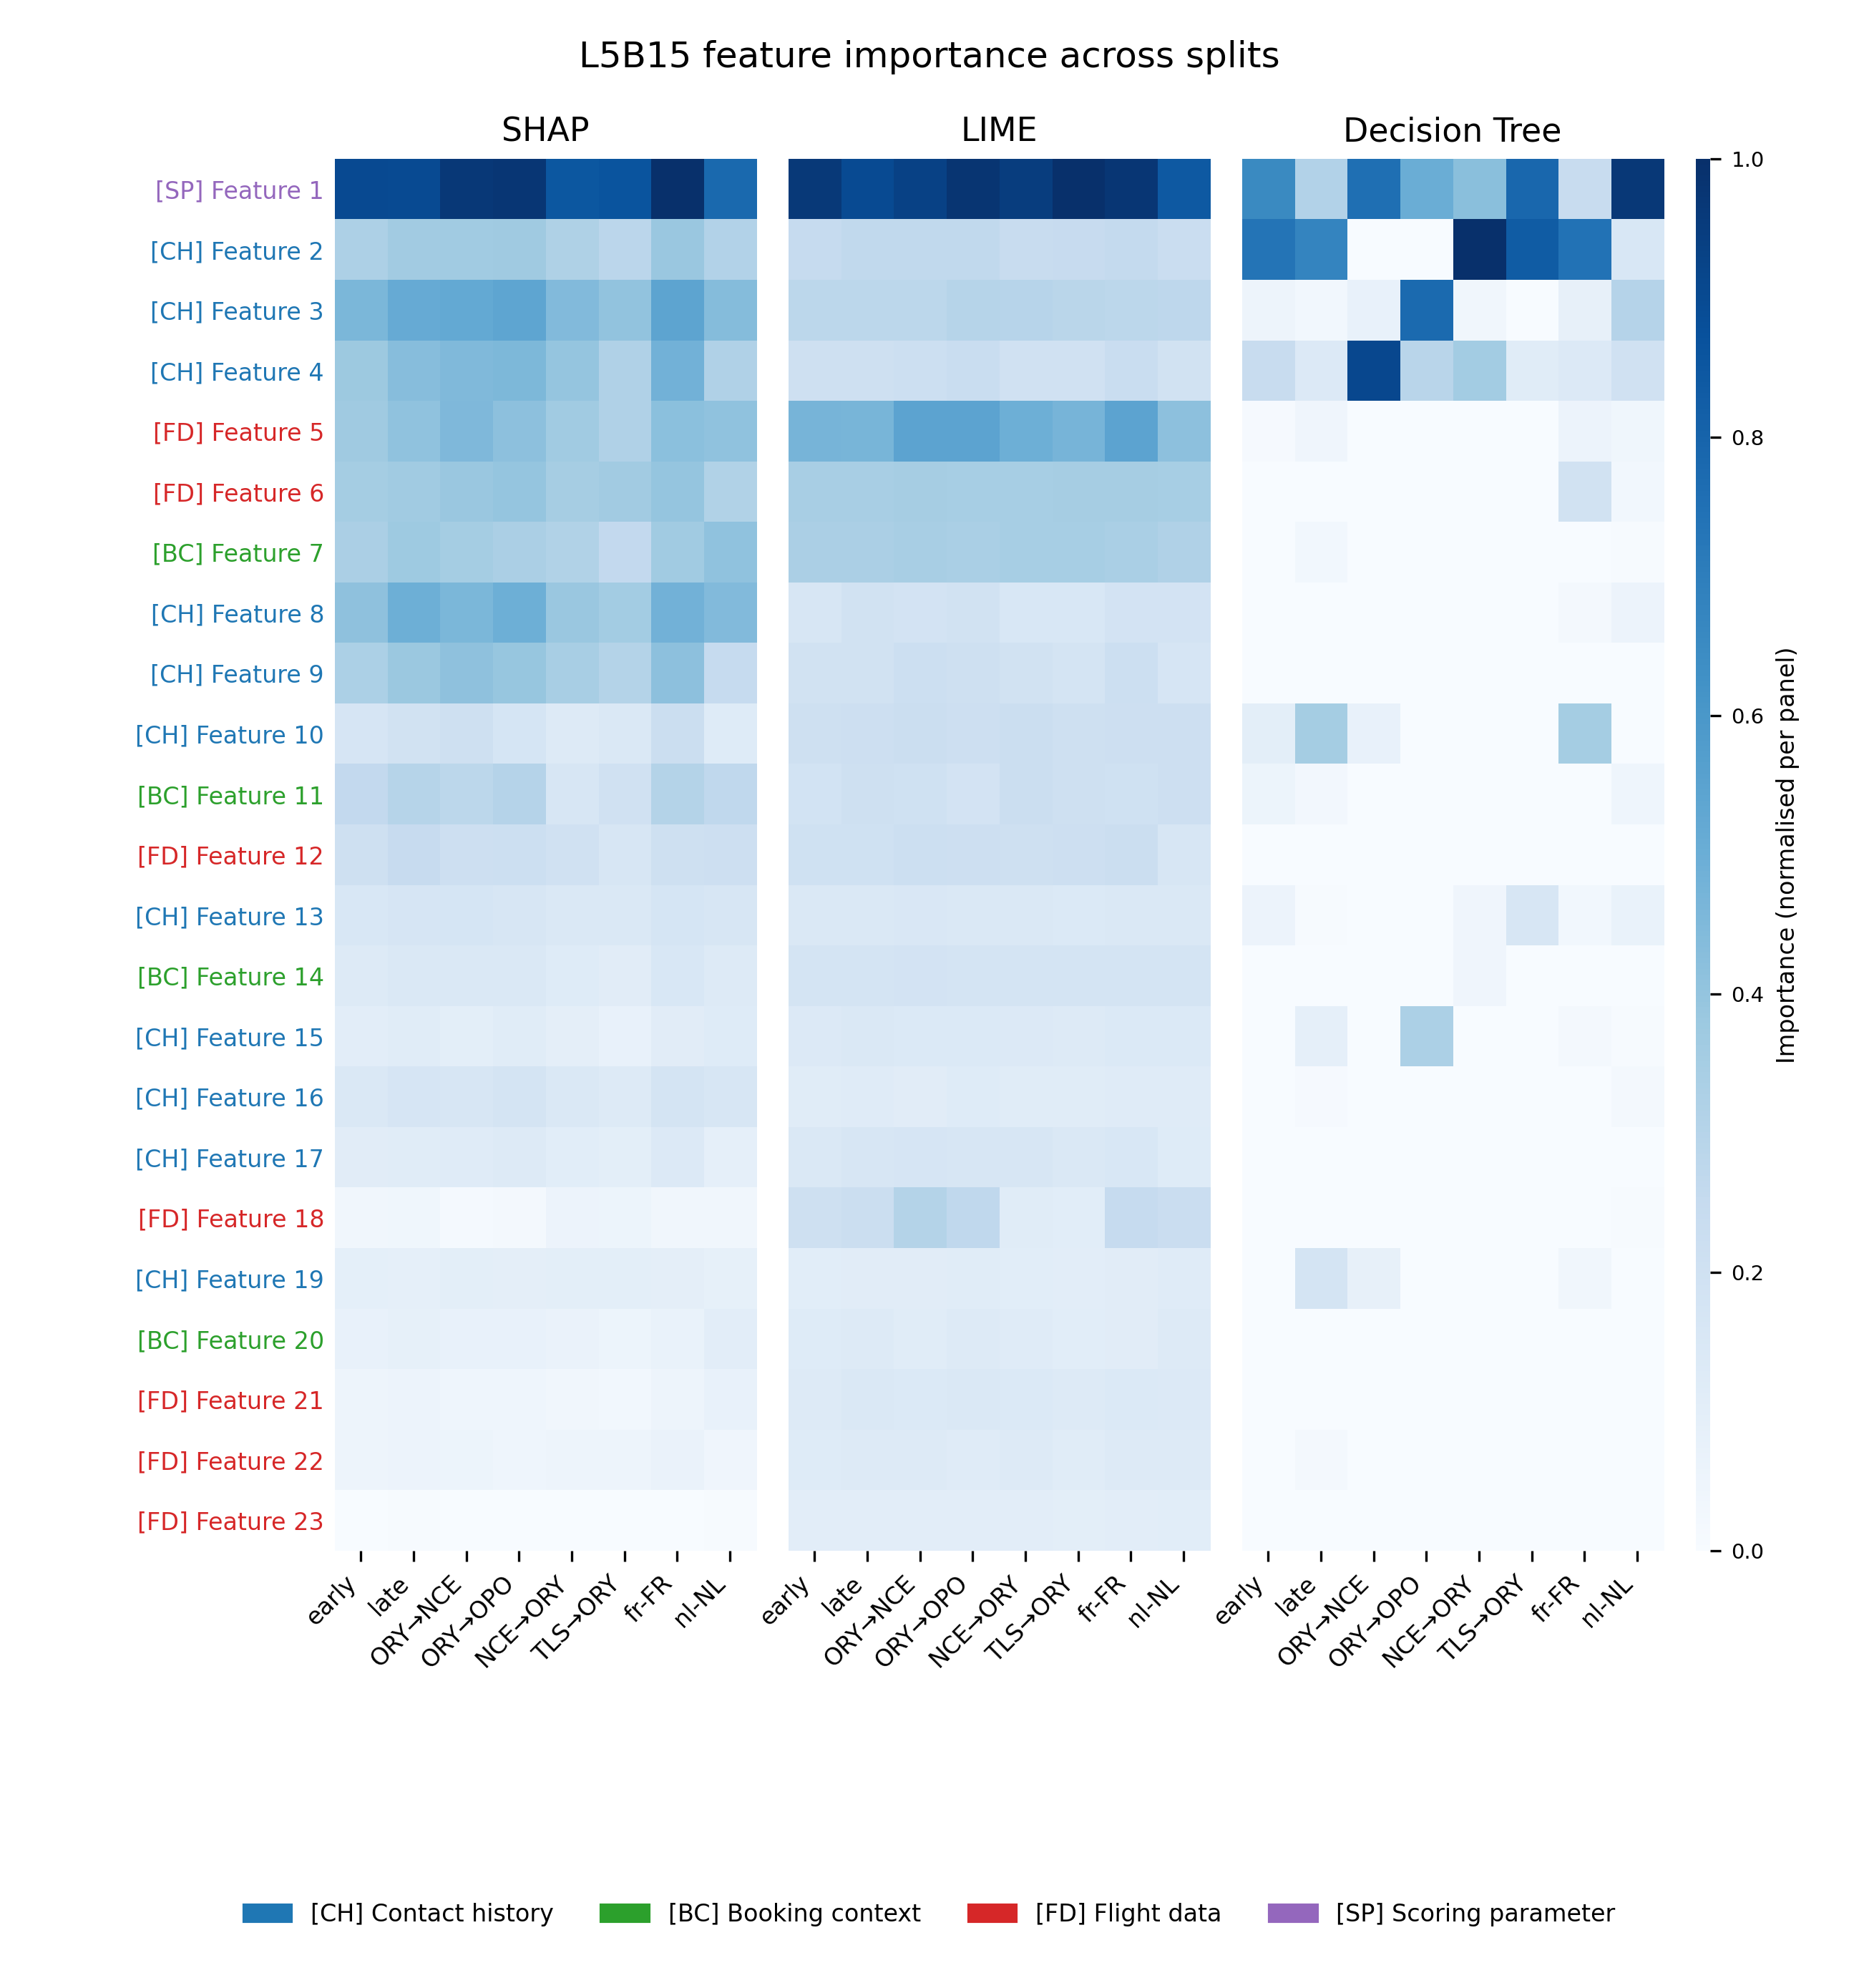
\includegraphics[width=\textwidth]{figures/feature_importance_heatmap_anonymised.png}
\caption{Normalised feature importance across L5B15 splits for SHAP, LIME, and the decision tree surrogate. Importance scores within each panel are normalised to $[0,1]$ by dividing by the panel maximum. Features are ordered by mean importance across all splits and methods, most important at top. Feature names are anonymised; features belong to four groups: contact history, booking context, flight data, and scoring parameters.}
\label{fig:feature_importance_heatmap}
\end{figure}

\section{Instability Attribution (RQ3)} \label{sec:rq3}

The stability values $\rho_{\text{DT}}$, $\rho_{\text{SHAP}}$, and $\rho_{\text{LIME}}$ underlying the decomposition below are reported in Table~\ref{tab:stability_l5b15}. Table~\ref{tab:attribution_l5b15} decomposes the observed instability into its component sources following the classification rule in Table~\ref{tab:attribution_rule}: For L5B15 the temporal split is classified as Both, and all four subgroup splits as Explainer.

\begin{table}
\caption{L5B15 instability attribution. $\delta_d$ is the Kolmogorov--Smirnov statistic on the propensity distribution; flagged if $\geq 0.10$. $\delta_m$ is the Jaccard overlap on the set of model versions active in each sub-population; flagged if $\leq 0.10$. $\delta_e^{\mathrm{DT}} = \rho_{\mathrm{SHAP}} - \rho_{\mathrm{DT}}$ and $\delta_e^{\mathrm{LIME}} = \rho_{\mathrm{SHAP}} - \rho_{\mathrm{LIME}}$ are the refit and sampling sensitivity gaps respectively; both are descriptive and not used for source classification. Source assignment follows Table~\ref{tab:attribution_rule}.}
\label{tab:attribution_l5b15}
\begin{tabular}{lrrrrl}
\toprule
Split & $\delta_d$ & $\delta_m$ & $\delta_e^{\mathrm{DT}}$ & $\delta_e^{\mathrm{LIME}}$ & Source \\
\midrule
L5B15 temporal & 0.356 & 0.002 & 0.141 & 0.007 & Both \\
Route pair 1 (ORY$\to$NCE vs ORY$\to$OPO) & 0.099 & 0.481 & 0.484 & 0.008 & Explainer \\
Route pair 2 (ORY$\to$OPO vs NCE$\to$ORY) & 0.094 & 0.547 & 0.406 & 0.132 & Explainer \\
Route pair 3 (NCE$\to$ORY vs TLS$\to$ORY) & 0.086 & 0.525 & 0.171 & -0.005 & Explainer \\
Culture (fr-FR vs nl-NL) & 0.081 & 0.595 & 0.291 & 0.009 & Explainer \\
\bottomrule
\end{tabular}
\end{table}


The temporal split is the only case where external conditions are significant: both the propensity distribution and the model snapshot pool shift substantially between the early and late window. Despite this, all three explanation methods remain relatively stable, with SHAP and LIME showing near-perfect rank preservation and the decision tree showing modest instability. The DT refit gap of the temporal split is the smallest across splits, indicating that when the underlying system shifts, the dominant features driving propensity scores remain largely the same regardless of explanation method. The feature importance structure is robust to external variation.

The four subgroup splits tell the opposite story. Both external diagnostics fall below their respective thresholds across all four splits: propensity distributions are stable and model snapshot overlap is high, confirming that these splits isolate the explanation methods from system-level changes. Yet the decision tree shows substantial ranking instability, with refit gaps ranging from 0.171 to 0.484, while SHAP rankings are near-perfect across all four splits. LIME tracks SHAP closely in three of the four splits, with a near-zero sampling sensitivity gap. The exception is the ORY$\to$OPO vs NCE$\to$ORY comparison, where LIME's sampling sensitivity rises to 0.132, suggesting that local perturbation sampling is more sensitive to the specific subgroup composition of that route pair. The within-route bootstrap validation confirms that the DT instability observed here reflects genuine subgroup sensitivity rather than random fitting noise: for three of the four subgroup splits the between-split $\rho_{\text{DT}}$ falls more than 0.10 below the within-sample mean, well exceeding the noise floor established by ten resamples on identical data (Appendix~\ref{app:bootstrap_dt}).

Taken together, these results answer RQ3 directly: under controlled conditions where external sources of variation are absent, the dominant source of observed instability is the explanation method itself. The decision tree is consistently the least stable method, driven by refitting variance rather than genuine model or data change. SHAP is the most stable across all splits, with LIME tracking it closely. Under large external shifts the decision tree continues to diverge from SHAP, although the magnitude of that divergence is smaller on the L5B15 temporal split ($\delta_e^{\mathrm{DT}} = 0.141$) than on its subgroup splits (0.171--0.484); SHAP and LIME continue to track each other closely throughout.

\section{Cross-Offer Replication (RQ4)} \label{sec:rq4}

RQ4 asks whether the fidelity and stability findings observed for the primary L5B15 luggage offer replicate across three further offer variants: CLUG (generic luggage), BookingDotCom (third-party accommodation), and Cartrawler (third-party car rental). The same surrogate-and-attribution pipeline is applied to each variant, with routes pinned to the L5B15 set for direct comparability and culture splits added where data permits. Surrogate fidelity per variant is reported in Table~\ref{tab:surrogate_fidelity_per_variant}; the per-variant instability attribution is reported in Table~\ref{tab:attribution_replication}.

\begin{table}[ht]
\caption{RQ4 replication: attribution summary for CLUG, BookingDotCom, and Cartrawler, grouped by split. Routes are pinned to the L5B15 set (ORY$\to$NCE, ORY$\to$OPO, NCE$\to$ORY, TLS$\to$ORY) for direct comparability. Metric definitions and thresholds match Table~\ref{tab:attribution_l5b15}: $\delta_d$ from the Kolmogorov--Smirnov statistic on propensity, flagged if $\geq 0.10$; $\delta_m$ from Jaccard overlap on the set of active model versions, flagged if $\leq 0.10$. $\delta_e^{\mathrm{DT}}$ and $\delta_e^{\mathrm{LIME}}$ are descriptive and not used for source classification.}
\label{tab:attribution_replication}
\centering
\begin{tabular}{lrrrrl}
\toprule
Variant & $\delta_d$ & $\delta_m$ & $\delta_e^{\mathrm{DT}}$ & $\delta_e^{\mathrm{LIME}}$ & Source \\
\midrule
\multicolumn{6}{l}{\textit{Temporal splits}} \\
CLUG & 0.390 & 0.002 & 0.421 & 0.005 & Both \\
BookingDotCom & 0.246 & 0.002 & 0.166 & 0.006 & Both \\
Cartrawler & 0.721 & 0.002 & 0.373 & 0.025 & Both \\
\midrule
\multicolumn{6}{l}{\textit{Route pair 1 (ORY$\to$NCE vs ORY$\to$OPO)}} \\
CLUG & 0.052 & 0.406 & 0.363 & 0.015 & Explainer \\
BookingDotCom & 0.116 & 0.416 & 0.711 & -0.036 & Dist. shift \\
Cartrawler & 0.079 & 0.404 & 0.512 & 0.009 & Explainer \\
\midrule
\multicolumn{6}{l}{\textit{Route pair 2 (ORY$\to$OPO vs NCE$\to$ORY)}} \\
CLUG & 0.116 & 0.404 & 0.266 & 0.197 & Dist. shift \\
BookingDotCom & 0.224 & 0.352 & 0.471 & -0.024 & Dist. shift \\
Cartrawler & 0.059 & 0.361 & 0.757 & 0.367 & Explainer \\
\midrule
\multicolumn{6}{l}{\textit{Route pair 3 (NCE$\to$ORY vs TLS$\to$ORY)}} \\
CLUG & 0.069 & 0.426 & 0.490 & 0.015 & Explainer \\
BookingDotCom & 0.062 & 0.396 & 0.333 & -0.010 & Explainer \\
Cartrawler & 0.062 & 0.376 & 0.571 & 0.010 & Explainer \\
\midrule
\multicolumn{6}{l}{\textit{Culture (fr-FR vs nl-NL)}} \\
CLUG & 0.114 & 0.464 & 0.383 & -0.017 & Dist. shift \\
BookingDotCom & 0.718 & 0.529 & 0.054 & -0.060 & Dist. shift \\
Cartrawler & 0.689 & 0.564 & 0.177 & 0.352 & Dist. shift \\
\bottomrule
\end{tabular}
\end{table}


\subsection{Surrogate Fidelity Across Variants}

Surrogate fidelity is reported in table~\ref{tab:surrogate_fidelity_per_variant}.The CatBoost surrogate achieves high pointwise fidelity on both luggage variants ($R^2 = 0.927$ on L5B15, $0.954$ on CLUG) and on Cartrawler ($R^2 = 0.912$); BookingDotCom is lower at $R^2 = 0.793$ despite its large sample, indicating that some BookingDotCom variance is not captured at the chosen surrogate depth. Rank fidelity (Spearman~$\rho$) is comparably strong on three of the four variants (0.92--0.95) but drops to $0.615$ on Cartrawler, meaning the surrogate reproduces Cartrawler's propensity ordering noticeably less faithfully than the other variants. This caveat is carried forward when reading Cartrawler's downstream attribution numbers: explanation diagnostics inherit the surrogate's approximation error and Cartrawler-specific results should be interpreted with the lower rank-fidelity baseline in mind.

\subsection{Temporal Split: Full Replication}

The temporal pattern observed for L5B15 replicates across all three additional variants. Every variant is classified as Both, indicating significant propensity drift ($\delta_d \geq 0.10$) accompanied by near-complete model-version turnover ($J_v < 0.005$) between the early and late observation windows. The magnitude of propensity drift varies substantially across variants, ranging from $\delta_d = 0.246$ on BookingDotCom to $0.721$ on Cartrawler (with L5B15 at $0.356$ and CLUG at $0.390$), yet the classification is identical because the model-version overlap is uniformly near zero. This is the expected consequence of Pega ADM's continuous online learning: any time window long enough to span meaningful population dynamics also spans many micro-updates of the underlying Naive Bayes, so temporal splits structurally combine data drift and snapshot turnover regardless of which offer is being scored. The DT refit-sensitivity gap $\delta_e^{\mathrm{DT}}$ is substantial across the temporal split for every variant (0.141--0.421) and is notably larger for CLUG and Cartrawler than for L5B15 itself, so the decision tree continues to diverge from SHAP under externally-driven shifts and not only under the controlled subgroup conditions of RQ3. By contrast, LIME sampling sensitivity stays near zero in all four variants (largest $\delta_e^{\mathrm{LIME}} = 0.025$ on Cartrawler), meaning LIME continues to track SHAP closely throughout. The pattern that emerges is consistent across split types: SHAP and LIME agree on the top-feature ranking whether the underlying instability is externally-driven or controlled, while the decision tree disagrees with both regardless of which source is driving the shift.

\subsection{Route Subgroups: Largely Replicates with Two Reclassifications}

Route subgroup splits replicate the L5B15 Explainer pattern across most cells, with reclassifications to Dist.\ shift on cells where $\delta_d$ marginally crosses the threshold. Route pair 3 (NCE$\to$ORY vs TLS$\to$ORY) is classified as Explainer for every variant including L5B15, with $\delta_e^{\mathrm{DT}}$ between 0.171 and 0.571 in every cell. Route pair 1 (ORY$\to$NCE vs ORY$\to$OPO) is Explainer for L5B15, CLUG, and Cartrawler; BookingDotCom alone flips to Dist.\ shift because its $\delta_d$ marginally crosses the threshold ($0.116$), even though its $\delta_e^{\mathrm{DT}}$ on this row is the largest in the entire table at $0.711$. Route pair 2 (ORY$\to$OPO vs NCE$\to$ORY) is Explainer for L5B15 and Cartrawler, and Dist.\ shift for CLUG ($\delta_d = 0.116$) and BookingDotCom ($\delta_d = 0.224$).

The qualitative interpretation of the RQ3 finding holds even on the reclassified rows: in every route pair and every variant, $\delta_e^{\mathrm{DT}}$ remains substantial (0.266--0.757), so the decision tree is concurrently contributing to ranking instability whether or not the external diagnostic crosses the threshold. The reclassifications to Dist.\ shift therefore do not reverse the Explainer story; they indicate that in some non-L5B15 route pairs the external trigger is also present alongside the explainer gap. LIME sampling sensitivity is small or slightly negative across most route cells, consistent with the L5B15 pattern, with one notable exception: Cartrawler route pair 2 shows $\delta_e^{\mathrm{LIME}} = 0.367$, indicating that LIME's local perturbation sampling is unusually unstable for that specific subgroup of Cartrawler.

\subsection{Culture Split: A Divergent Finding}

The culture split is the one place where the L5B15 finding does not replicate. L5B15 is classified as Explainer because its culture-driven propensity shift sits just below the threshold ($\delta_d = 0.081$). All three replication variants flip to Dist.\ shift: CLUG shows a modest above-threshold shift ($\delta_d = 0.114$), and BookingDotCom and Cartrawler show very large shifts ($\delta_d = 0.718$ and $0.689$ respectively). The substantive reading is that customer culture (French versus Dutch) maps onto materially different propensity distributions for the cross-sell and third-party offers but not for the luggage upsell. That is, the Pega model has learned a stronger culture-conditional response pattern in BookingDotCom and Cartrawler than in the luggage offers, plausibly because accommodation and car-rental preferences vary more across European customer segments than basic luggage add-on uptake does.

The two third-party variants also produce instructive explainer-gap patterns under culture. BookingDotCom's $\delta_e^{\mathrm{DT}}$ collapses to $0.054$ on the culture split, the lowest in the entire table, meaning that despite a very large external shift the decision tree's ranking is comparatively stable across cultures for that variant. Cartrawler shows the opposite pattern, with $\delta_e^{\mathrm{LIME}} = 0.352$ alongside its large $\delta_d$, indicating that LIME's local sampling becomes unstable in the same comparison that also exhibits substantial external drift. These two cells illustrate that even when external sources fire, the relative contribution of refit and sampling sensitivity can vary substantially across product contexts.

\subsection{Summary of Replication Evidence}

The replication evidence supports the RQ3 conclusion with one important caveat. The temporal pattern of externally-driven instability with moderate DT contribution replicates fully across all four variants. The route pattern of explainer-dominant instability under controlled same-window conditions replicates qualitatively across all variants, with three rows reclassified to Dist.\ shift on borderline $\delta_d$ values; the underlying DT-versus-SHAP gap remains the larger numerical contributor in those cells. The culture pattern does not replicate: L5B15 culture instability is classifiable as Explainer-driven only because its $\delta_d$ sits just below threshold, whereas the three other variants exhibit genuine culture-induced propensity shifts large enough to dominate the attribution. This divergence is best read as a property of the underlying Pega model rather than of the evaluation pipeline: customer culture has a stronger effect on third-party and generic-luggage propensity than on the L5B15 weight-specific luggage offer. The methodological findings therefore generalise, while the substantive role of any one feature dimension in driving observed instability is product-context-specific.


\section{Feature Drivers and Business Implications (RQ5)} \label{sec:rq5}

§\ref{sec:rq2} established that the three explanation methods converge on the same L5B15 attribution structure at the level of feature groups across every split tested, even where their individual feature ranks diverge, and §\ref{sec:rq3} attributed the residual individual-rank drift to decision-tree refit variance ($\delta_e^{\mathrm{DT}}$) rather than to underlying model or data change. Together those two results licence reading group-level attribution shares as a substantive description of what the production model has learned to score on, regardless of which of the three methods supplies them. This section takes that licence and asks the content question: which features drive the L5B15 propensity score, and what the resulting attribution structure means for the marketing and governance stakeholders who consume those scores.

\subsection{What the Model Scores On}

Table~\ref{tab:rq5_feature_importance} reports the per-feature importance share for each method, ordered by mean rank across the three. Beyond the offer-identity scoring parameter, which carries the single largest share in every method as expected for a feature that encodes which product is being scored, the highest-ranked predictors are overwhelmingly contact-history features: the number of days since the last outbound email and the historical count of prior outbound contacts. These are recency and frequency signals, the two quantities that together define contact fatigue. The decision tree concentrates an especially large share on a single such feature, the historical outbound-email count, consistent with its tendency to split early on whichever recency or frequency variable is most discriminative.

\begin{table}[ht]
\caption{L5B15 feature-importance shares across the three explanation methods, ordered by the SHAP/LIME consensus rank (the mean of the SHAP and LIME within-method ranks). The ordering uses only the two methods that RQ2 and RQ3 found reliable; the decision-tree share is reported as a corroborating column but does not drive the ordering. Each method's importances are normalised to sum to 100\%. Group tags: CH~=~contact history, FD~=~flight data, BC~=~booking context, SP~=~scoring parameter.}
\label{tab:rq5_feature_importance}
\centering
\small
\begin{tabular}{llrrrr}
\toprule
Feature & Grp & SHAP\% & LIME\% & DT\% & SL rank \\
\midrule
Param.BundleName & SP & 15.7 & 19.0 & 21.5 & 1.0 \\
Email.Out.Pending.DaysSinceLast & CH & 8.5 & 5.5 & 2.2 & 3.5 \\
SeatNumber & FD & 6.9 & 10.3 & 2.3 & 3.5 \\
IsStaffStandBy & FD & 6.4 & 7.1 & 0.0 & 4.5 \\
Email.Out.Delivered.DaysSinceLast & CH & 7.1 & 4.0 & 10.1 & 5.5 \\
BookingMonth & BC & 6.1 & 6.7 & 1.6 & 6.0 \\
Email.Out.Pending.HistCount & CH & 6.0 & 4.8 & 34.5 & 7.5 \\
Push.Out.Pending.LastGroup & CH & 8.0 & 3.1 & 0.2 & 8.5 \\
Email.Out.Pending.LastGroup & CH & 6.2 & 3.3 & 0.0 & 10.0 \\
FlightInboundArrival & BC & 4.9 & 3.8 & 1.1 & 10.0 \\
Language & FD & 4.0 & 3.8 & 0.1 & 10.0 \\
Email.In.Clicked.DaysSinceLast & CH & 2.9 & 3.5 & 17.0 & 11.5 \\
BookerGender & BC & 2.4 & 3.5 & 1.3 & 13.5 \\
Push.Out.Pending.DaysSinceLast & CH & 2.8 & 2.5 & 2.2 & 14.0 \\
DestinationAirport & FD & 0.6 & 3.9 & 0.0 & 15.0 \\
Event.Out.RealTimeEvent.HistCount & CH & 2.8 & 1.9 & 0.0 & 16.5 \\
Email.Out.Delivered.LastGroup & CH & 2.0 & 2.3 & 0.0 & 16.5 \\
AirlineCodeIATA & FD & 0.9 & 2.4 & 0.0 & 18.0 \\
Email.In.Pending.DaysSinceLast & CH & 1.9 & 1.8 & 1.0 & 18.5 \\
Journey & FD & 0.9 & 1.9 & 1.2 & 19.5 \\
Push.Out.Pending.HistCount & CH & 1.6 & 1.5 & 3.6 & 20.0 \\
CultureCode & BC & 1.4 & 1.8 & 0.1 & 20.0 \\
FlightNumberOperatorIATA & FD & 0.1 & 1.3 & 0.0 & 23.0 \\
\bottomrule
\end{tabular}
\end{table}


\subsection{Recency and Fatigue, Not Customer Identity}

Aggregated to the feature-group level (Table~\ref{tab:rq5_group_importance}), the pattern is unambiguous. Contact-history features account for roughly half of total importance under SHAP and for the large majority under the decision tree; flight-level features form the second pillar. Booking context and the scoring parameter make up the remainder. Customer-level attributes, demographics and loyalty profile, contribute nothing, because no customer attribute survives Pega's active-predictor selection for L5B15 in the first place (Section~\ref{sec:data}).

\begin{table}[ht]
\caption{L5B15 feature-importance aggregated by feature group, as a percentage of each method's total importance. Contact-history (recency and frequency of prior outbound contact) and flight-level features dominate across all three methods; customer-level attributes contribute nothing because none survive Pega's active-predictor selection for L5B15.}
\label{tab:rq5_group_importance}
\centering
\begin{tabular}{llrrr}
\toprule
Feature group & \# feat & SHAP\% & LIME\% & DT\% \\
\midrule
Contact history & 11 & 49.8 & 34.4 & 70.8 \\
Flight data & 7 & 19.7 & 30.7 & 3.6 \\
Booking context & 4 & 14.8 & 15.8 & 4.1 \\
Scoring parameter & 1 & 15.7 & 19.0 & 21.5 \\
\midrule
Customer attributes & 0 & 0.0 & 0.0 & 0.0 \\
\bottomrule
\end{tabular}
\end{table}


The commercial reading is direct. For this offer, the propensity model is, in effect, scoring how recently and how often the customer has been contacted, together with the context of the booked trip, rather than who the customer is. Loyalty tier, demographics, and historical value, the attributes marketing teams most often assume drive personalisation, play no role in the L5B15 score because they were never retained as predictors. The actionable lever this surfaces is contact strategy: because recency and contact-frequency dominate the score, the model's behaviour is highly sensitive to the cadence of the outbound programme itself, and a frequency-capping or fatigue-management policy would move propensities more reliably than richer customer segmentation. This also tempers a common governance expectation: an audit asking ``which customer characteristics drive this offer?'' would find that, for L5B15, the honest answer is essentially none.

\subsection{A Top Predictor Encoding Missingness, Not Value}

One flight-group predictor warrants separate scrutiny. The staff-standby flag, which marks bookings issued on a staff standby ticket, ranks among the most important features under both SHAP and LIME (Table~\ref{tab:rq5_feature_importance}), which is commercially counter-intuitive: staff standby travel should have little to do with a passenger's propensity to buy a luggage add-on. Inspection of the raw field explains the anomaly. The flag is almost never true; what varies across records is whether the field is populated at all. Table~\ref{tab:rq5_staffstandby_proxy} shows that records for which the field is populated are far more likely to carry a previous-flight customer profile than records for which it is blank ($20.3\%$ versus $3.0\%$, a $6.8\times$ difference; point-biserial $r = 0.25$ and Cram\'er's $V = 0.25$ with the presence of a previous-flight profile, both $p \approx 0$).

\begin{table}[ht]
\caption{Test of the missingness-proxy hypothesis for \texttt{IsStaffStandBy} on L5B15. The flag is never \texttt{true} in the sample, and what varies across records is whether the field is populated at all; where it is populated, customer-profile data is far more likely to be present, indicating that the surrogate (and the underlying model) keys on the field's \emph{presence} as a proxy for record completeness rather than on staff/standby status itself.}
\label{tab:rq5_staffstandby_proxy}
\centering
\begin{tabular}{lr}
\toprule
Quantity & Value \\
\midrule
n (L5B15 records) & 64,006 \\
IsStaffStandBy populated rate & 0.582 \\
P(IsStaffStandBy = True) overall & 0.0000 \\
P(IsStaffStandBy = True | populated) & 0.0000 \\
customer fields in $C$ (excl.\ prev-flight) & 75 \\
previous-flight fields in $Y$ & 33 \\
mean customer-completeness | populated & 0.755 \\
mean customer-completeness | blank/null & 0.714 \\
P(previous-flight profile | populated) & 0.203 \\
P(previous-flight profile | blank/null) & 0.030 \\
risk ratio & 6.8x \\
point-biserial r (populated vs completeness) & 0.251 (p=0.0e+00) \\
Cramér's V (populated vs prev-flight profile) & 0.253 (p=0.0e+00) \\
\bottomrule
\end{tabular}
\end{table}


The predictor is therefore acting as a proxy for record completeness rather than for staff-standby status: its populated-ness co-varies with whether the customer is a recognised returning traveller with historical profile data attached. This is the visible downstream symptom of Pega's predictor selection. Because the platform deactivates sparse customer-level predictors and retains only the strongest of any group of correlated predictors, the missingness pattern those predictors would have carried does not disappear; it re-emerges, encoded in the presence pattern of a surviving feature that happens to correlate with data availability. The governance implication is concrete and transferable: in a continuously self-selecting feature space, a feature's measured importance can reflect which records have data rather than what the data says, and a predictor that an audit would flag as nonsensical may in fact be the model's handle on an unmodelled missingness structure. Detecting this requires checking high-importance predictors against their own populated-ness, a cheap diagnostic that this case study shows is worth running before attribution results are presented to stakeholders.

\chapter{Discussion} \label{Discussion}

\section{Summary of Key Findings}

Across the five research questions the empirical picture is internally consistent. A CatBoost surrogate reproduces Pega ADM's logged propensity scores with high rank fidelity on three of the four offer variants studied, providing a sufficient base for downstream attribution. Built on that surrogate, SHAP and LIME produce highly stable feature rankings across temporal, route, and customer-culture splits, while a shallow decision tree surrogate fitted directly on the propensities produces rankings that vary substantially between subgroups. The instability-attribution diagnostic shows that under controlled same-window conditions, where neither the propensity distribution nor the active model snapshots shift meaningfully, the dominant source of observed ranking instability is the explanation method itself. The pattern replicates across three further offer variants on temporal and route splits; the one place L5B15 diverges from the replication set is the customer-culture split, where the third-party offers exhibit substantial culture-conditional propensity shifts that the luggage variant does not.

Across explanation methods, SHAP is the most reliable in this setting. LIME tracks SHAP closely with one exception linked to its local perturbation sampling. The decision tree surrogate, despite being interpretable in the strictest end-to-end sense, is the least stable across populations even when the underlying model has not changed.

\section{Interpretation of Findings by Research Question}

\subsection{Surrogate Fidelity (RQ1)}

The fidelity result is, in one reading, unsurprising: a flexible gradient-boosted ensemble trained directly on logged scores ought to reproduce those scores reasonably well. What matters here is not the level itself but its consequence for the rest of the pipeline. Because SHAP and LIME operate on the surrogate $g$, every attribution they emit is downstream of $g$'s approximation of $f$. The decision tree surrogate, fitted directly on $p$, faces a single layer of approximation rather than two. Strong rank fidelity on three of four variants is therefore the condition that licenses attribution claims for SHAP and LIME in those settings, not a free-standing result.

The Cartrawler exception illustrates the practical importance of reporting rank-based fidelity alongside $R^2$. Cartrawler's pointwise fit is comparable to the other variants, yet its Spearman rank correlation is markedly lower. The surrogate captures Cartrawler's propensity scale but reproduces its ordering less faithfully. For a system that consumes propensities through prioritisation rather than calibration, the rank disagreement is the more consequential one. Downstream attribution results for Cartrawler are accordingly interpreted with that fidelity caveat, not as evidence on equal footing with the other variants.

The candidate-model comparison underlying the architecture choice also has interpretive value. A Gaussian Naive Bayes baseline, architecture-matched to Pega's internal model, lags behind every tree-based candidate on the fidelity suite. This is consistent with the broader observation in the XAI literature that an explanation pipeline constrained to the black-box model's own functional class is not necessarily the best surrogate of its input-output behaviour, particularly when feature interactions and high-cardinality categoricals are involved \parencite{molnar_interpretable_2025}. A flexible surrogate produces more faithful approximations to the model output, even when the underlying model is itself a simpler classifier. In the present setting, two factors plausibly drive this gap. First, Pega ADM's online learning produces a continuously evolving Naive Bayes that, viewed as a single input-output function over the observation window, behaves like a mixture rather than a single classifier; a flexible surrogate captures the mixture more faithfully than any single-snapshot Naive Bayes can. Second, Pega's bin-based handling of categoricals collapses information that CatBoost's native ordered target encoding preserves.

\subsection{Explanation Stability (RQ2)}

The stability results sharpen one of the central concerns of the XAI evaluation literature: explanations of the same model can diverge across populations even when the populations are drawn from the same data-generating process \parencite{ribeiro_why_2016, vilone_explainable_2020}. The contribution here is to show how that divergence behaves across three explanation families under deliberately controlled conditions.

SHAP's high stability is structurally expected. Because a single CatBoost surrogate is fitted once on the full training set and applied to both sub-populations of every split, TreeSHAP's deterministic computation leaves no room for refitting variance. Any observed ranking shift reflects only how the surrogate weighs features differently in different sub-populations. That this shift remains small across temporal, route, and culture splits indicates that the surrogate's attribution structure is itself stable, not just that the method is deterministic.

LIME's close tracking of SHAP is more notable than it might appear at first reading. LIME shares the fixed-surrogate property with SHAP but introduces an additional source of variance through its perturbation-based local linear fits. That LIME nevertheless matches SHAP's stability on most splits suggests that the sampling variance is modest in practice for this dataset and feature space. The exception on the route pair with neither shared origin nor destination shows that this is not guaranteed: when two sub-populations share no structural element, local linear approximations can shift enough to move global aggregates.

The decision tree's instability is the central finding of RQ2. A shallow tree concentrates importance on whichever single feature is most discriminative in a given subgroup, rather than distributing it across the active feature set; small changes in subgroup composition can therefore reshuffle the top of the ranking even when the model is not asked to change. This is a property of tree-based importance more than of decision trees as such, and it has been documented in the broader interpretable-machine-learning literature \parencite{molnar_interpretable_2025}, but the magnitude observed here is substantial. The bootstrap validation rules out the alternative explanation that this is fitting noise: on three of four subgroup splits the between-split disagreement exceeds within-split disagreement by margins well outside what re-fitting on the same data can produce.

For a production decisioning system the operational implication is direct. A practitioner who inspects per-subgroup decision-tree explanations to understand why a model behaves differently on different customer segments may attribute that difference to the model itself, when in fact the underlying scoring function has barely moved and the difference lies in how the explanation method aggregates importance over the subgroup. Stability of an explanation is therefore not only a property of the model being explained; it is a property of the explanation method, the surrogate where one is used, and the interaction between the two and the evaluation data.

\subsection{Instability Attribution (RQ3)}

The instability-attribution diagnostic operationalises a question implicit in much of the XAI evaluation literature but rarely answered directly: when explanations of a deployed model disagree across populations, where does the disagreement come from \parencite{vilone_explainable_2020, molnar_interpretable_2025}? The three-source decomposition, distribution shift $\delta_d$, model churn $\delta_m$, and explainer sensitivity $\delta_e$, separates causes that are commonly conflated and provides a structured basis for assigning observed instability to its dominant source.

The L5B15 temporal split is the only case where both external sources fire simultaneously: the propensity distribution shifts substantially across the observation window, and model-snapshot overlap collapses to near zero. This is not a flaw of the split design but a structural property of continuous online learning. Any time window long enough to span meaningful population dynamics will also span many micro-updates of the underlying Naive Bayes. The temporal split therefore mixes data drift and snapshot turnover by construction, and a clean separation between the two in the temporal case is not available from observational logs alone.

The same-window subgroup splits, route and culture, are the test cases where the diagnostic does most of its work. Because those splits share an observation window, both $\delta_d$ and $\delta_m$ are constrained to be small by design; any remaining ranking instability isolates the contribution of the explanation method. On every same-window split for L5B15 the decision tree's refit gap is substantial, SHAP rankings remain near-identical, and LIME tracks SHAP within sampling tolerance. The conclusion is therefore not that decision-tree-based explanations are inherently unreliable, but rather that under operationally realistic conditions where data and model are approximately stable, the choice of explanation method materially affects which features appear to drive scoring.

A reader familiar with the XAI literature will note that the diagnostic does not claim causal identification. The three sources are proxied by effect-size statistics, not isolated by intervention, and $\delta_d$ and $\delta_m$ are themselves correlated, since the same incoming response data that shifts the feature distribution also drives the online updates. The protocol is best read as an indicative decomposition that surfaces distinctions normally collapsed inside a single instability number, not as a causal account of why a particular ranking moved.

\subsection{Cross-Offer Replication (RQ4)}

The replication evidence has both methodological and substantive readings. Methodologically, the protocol generalises: applying the same surrogate fitting, fidelity assessment, and attribution diagnostic to three further offer variants reproduces the qualitative pattern from L5B15 in nearly every cell. Temporal splits classify as Both across all four variants, route splits classify predominantly as Explainer with a small number of reclassifications to Dist.\ shift on borderline values of $\delta_d$, and the decision tree's refit gap remains the largest numerical contributor in route cells even when the formal classification flips. A practitioner applying this diagnostic to a new offer in the same CDH environment should expect to recover comparable patterns.

The substantive reading is more nuanced and is, in some ways, the more interesting result. The culture split is the one place where L5B15 does not replicate, but the divergence is not a failure of the protocol. L5B15's customer-culture propensity shift sits just below the $\delta_d$ threshold, while the three replication variants cross it. For BookingDotCom and Cartrawler the magnitude is large; for CLUG it is modest. The interpretation is that customer culture, in this study French versus Dutch, maps onto materially different propensity distributions for the cross-sell and third-party offers but not for the L5B15 weight-specific luggage upsell. This is best read as a property of the underlying Pega model and the data it has accumulated on each offer, rather than of the evaluation pipeline.

The distinction between the methodological protocol generalising and the substantive feature-level effect being product-context-specific is one of the contributions of including offers from different commercial categories in the replication set rather than only weight-variant luggage offers. A cross-domain replication would also have validated the protocol, but would have offered less information about the diagnostic's behaviour on offers that share most of the feature space but differ substantively in customer-side response patterns.

\subsection{Feature Drivers (RQ5)}

The feature-level findings are, for a practitioner audience, the most directly consequential of the thesis. Two results stand out. The first is that the L5B15 propensity score is driven by contact recency and frequency and by the context of the booked trip, and not at all by customer identity. This is not a quirk of attribution but a structural consequence of how the model was built: Pega's predictor selection retained no customer-level attribute for this offer, so demographics and loyalty profile cannot drive the score regardless of which explanation method is used. The reading that the model scores contact fatigue more than it scores the customer is therefore robust to the explainer-stability concerns raised in RQ2 and RQ3, because it holds at the feature-group level where all three methods agree.

The second result is that a feature's importance can be an artefact of the data-collection process rather than a behavioural signal. The staff-standby predictor is influential not because staff-standby status predicts luggage purchase but because the field's populated-ness proxies for record completeness, and completeness in turn correlates with being a recognised returning customer. This is a specific, measured instance of a general hazard in self-selecting feature spaces: when a platform deactivates sparse predictors and groups correlated ones, the missingness structure those predictors carried is not removed but displaced onto whichever surviving feature correlates with data availability. The finding does not undermine the explanation methods, all three of which faithfully report that the model relies on the feature; it shows that faithful attribution and behavioural meaning are distinct, and that the gap between them is exactly where a data artefact can hide.

\section{Academic Implications}

The thesis contributes at two related levels to the XAI evaluation literature.

The first contribution is methodological: a structured instability-attribution protocol that decomposes observed explanation ranking shifts into three sources, using a pair of effect-size diagnostics applied directly to the propensity score distribution and the active-snapshot set. The decomposition is approximate rather than causal, and the chapter is explicit on that point, but it surfaces a class of distinctions that the existing XAI evaluation literature \parencite{vilone_explainable_2020, molnar_interpretable_2025} typically does not make. The combination of the Kolmogorov--Smirnov statistic on the model output distribution alongside Jaccard overlap on the set of active model-version identifiers has not, to my knowledge, previously been operationalised inside a CDH evaluation framework.

The second contribution is empirical: a systematic comparison of SHAP, LIME, and a decision-tree surrogate applied to Pega ADM propensity scores under production conditions, including continuous online updating, observational exposure-biased data, categorical-heavy feature spaces, and restricted model access. Standard XAI benchmarks evaluate methods on i.i.d.\ static datasets with full model access \parencite{molnar_interpretable_2025}; this thesis reports XAI behaviour under the inverse of those assumptions. The contribution is to document what changes, what does not, and which evaluation choices matter most when those assumptions are dropped.

A further methodological observation concerns the choice of surrogate architecture. The candidate-model comparison shows that an architecture-matched Naive Bayes surrogate is not the best approximator of an online-updating Naive Bayes black-box model. This points to a small but practically relevant gap in the existing surrogate-modelling literature, which tends to recommend functional-class matching as a default \parencite{molnar_interpretable_2025}.

\section{Practical Implications}

For organisations deploying explainability tooling on Pega ADM or similar continuously-updating CDH systems, five implications follow.

First, the choice of explanation method matters operationally, not only academically. Decision-tree surrogates are often preferred in governance contexts because they are interpretable end-to-end. The results in this thesis show that the same surrogate can produce substantially different feature rankings on subgroups of the same population even when the underlying model has not changed. Practitioners who rely on per-subgroup decision-tree explanations for compliance or audit purposes should be aware that the resulting story can be inconsistent across populations for reasons that have nothing to do with model behaviour. SHAP and LIME, despite their own theoretical limitations, are consistently more stable in the present setting.

Second, the instability-attribution diagnostic is directly deployable for monitoring. The two effect-size statistics underlying the diagnostic, the Kolmogorov--Smirnov statistic on logged propensity and the Jaccard overlap on the active model-version set, are cheap to compute from existing decisioning logs and require no access to ADM internals. A monitoring pipeline that tracks these alongside per-window explanation rankings would flag instability events and indicate, before any deep diagnostic work, whether the likely source is data drift, model turnover, the explanation method itself, or some combination.

Third, the surrogate-based explanation pipeline as a whole is a workable approach for practitioners without access to ADM internals. The Pega CDH platform does not currently expose a live scoring API for offline analysis, and the model's own internal predictor importances are accessible only through the Health Check predictor overview rather than through a queryable interface. The pipeline operationalised in this thesis, surrogate fitted on logged $(\mathbf{X}, p)$ tuples, fidelity assessed against the same logs, attributions explained on the surrogate, demonstrates that meaningful explanation work is possible inside that constraint. It does not replace direct ADM access where that is available; it provides a defensible second-best for the common case where it is not.

Fourth, the feature-driver findings reframe where personalisation effort is best spent for this offer. Because the propensity score is dominated by contact recency and frequency rather than by customer attributes (Section~\ref{sec:rq5}), the score responds more to the cadence of the outbound programme than to customer segmentation. A practical consequence is that a contact-frequency or fatigue-management policy, governing how recently and how often a customer has been emailed, is likely to shift propensities more reliably than investment in richer customer features, at least until customer-level predictors accumulate enough evidence to be activated. Marketing stakeholders expecting the model to key on loyalty tier or demographics should be told plainly that, for this offer, it does not.

Fifth, high-importance predictors should be checked against their own populated-ness before attribution results are presented for audit. The staff-standby case shows that in a self-selecting feature space a predictor can rank highly because its presence proxies for record completeness rather than because it carries behavioural signal. This is cheap to detect, comparing the missingness pattern of a top predictor against the availability of the deactivated features, and doing so guards against the governance failure mode in which a model is certified on an explanation that is faithful to the model but misleading about the world. More broadly, it argues for treating predictor deactivation and correlation grouping as first-class metadata in any CDH explanation review, since they determine which signals a feature is silently standing in for.

\section{Limitations}

A number of limitations qualify the interpretation of these findings.

The most fundamental is the double approximation that the explanation pipeline introduces. SHAP and LIME do not explain the production model $f$ directly; they explain the surrogate $g$ that approximates $f$. Explanation validity is therefore bounded by surrogate fidelity, and any region of the feature space where $g$ diverges from $f$ is a region where the resulting attributions may not faithfully describe Pega's behaviour. The fidelity assessment in Chapter~\ref{ch:results} establishes that $g$ approximates $f$ well in aggregate for three of the four variants studied, but does not certify pointwise fidelity for every input. The Cartrawler variant in particular sits below the level at which downstream attribution claims should be made with confidence; its results are reported and replicated, but their interpretive weight is correspondingly lower. The decision-tree surrogate sidesteps one layer of approximation by fitting directly on $p$, but at the cost of a much coarser representation of $f$ and the structural ranking instability documented above. Neither path is approximation-free, and the trade-off between fidelity layers and explanation interpretability is itself part of the methodological lesson of the thesis.

A related limitation is the encoding mismatch between the surrogates. The decision tree is implemented through scikit-learn and therefore uses ordinal encoding of categorical features, whereas CatBoost handles them natively. The decision-tree-versus-SHAP gap reported as $\delta_e^{\mathrm{DT}}$ partly reflects this encoding difference, and the methodology chapter is explicit that the gap is best interpreted as a composite of explainer sensitivity and encoding sensitivity rather than as a pure explainer effect.

A second class of limitations concerns the data and setting. The study is conducted within a single European airline, on the Email and Outbound channel only, and on a small portfolio of offers concentrated around luggage upsells with two third-party partner offers as replication. The replication design provides a meaningful generalisation check across offers within one CDH installation but does not constitute cross-industry or cross-channel validation. Findings should be interpreted as evidence about XAI method behaviour under the specific conditions of this production environment, with implications for practitioners operating in similar settings rather than as universal claims about explanation methods.

A third class of limitations concerns observational structure. All evaluation data is drawn from logged decisioning events, with no ability to query the live ADM scorer on counterfactual or held-out inputs. Exposure bias is intrinsic to the data: customers respond only to offers they were shown, and both the propensities and the explanations of those propensities are conditioned on the historical decisioning policy \parencite{lundberg_be_2018}. A deployment-time evaluation, in which the surrogate-and-attribution pipeline is run alongside the live ADM and fed with the same inputs in real time, would tighten some of the current claims; that was outside scope given access constraints.

Two narrower limitations are worth flagging. The Jaccard overlap on model-version identifiers proxies snapshot turnover rather than parameter shift directly: Pega ADM issues a new identifier on every micro-update, so two functionally identical snapshots can carry different IDs. This is mitigated by the structural property that same-window splits draw from the same active snapshot pool, but it remains an imperfect proxy. Separately, LIME importance rankings are aggregated across instances by averaging per-instance linear coefficients, which assumes coefficient comparability across the feature space; the conclusions on LIME stability should be read with that assumption in mind.

\section{Future Research}

Several extensions follow naturally from the results and the limitations.

A direct next step is to incorporate Pega ADM's own predictor importance signal as an external reference. The platform exposes per-predictor univariate AUC and bin-level lifts through its Health Check predictor overview. These quantities are not, strictly, explanations of an individual scoring event, but they do provide a model-internal view of which predictors carry evidential weight, and they can serve as a soft reference ranking against which the surrogate-based SHAP, LIME, and decision-tree attributions can be compared. Such a comparison was deliberately held outside the scope of this thesis to preserve the black-box framing on which the methodology rests, but it would constitute a valuable validation step in subsequent work, particularly for the cross-offer replication where surrogate fidelity varies.

A second direction is cross-channel and cross-industry replication. The present results cover Email and Outbound only and one airline; replicating the protocol on web, push, or mobile channels, and on CDH installations in other industries such as telecommunications, retail, or financial services, would test whether the patterns documented here are properties of CDH systems generally or of the airline luggage portfolio specifically.

A third direction concerns longitudinal evaluation. The temporal splits in this study compare early and late halves of a single observation window. A longer-horizon study, with multiple sequential splits across months or quarters, would permit assessment of whether explanation rankings drift coherently or chaotically over time, and whether the instability-attribution diagnostic produces stable classifications across rolling windows. This would also create the opportunity to incorporate formal concept-drift tests on the feature-level distributions, alongside the propensity-output diagnostic used here.

Counterfactual explanation methods and real-time explanation systems are natural complementary directions. Counterfactual approaches \parencite{molnar_interpretable_2025} provide explanations of the form ``the minimal change to the input that would have changed the decision''; they are a complement to the feature-attribution methods evaluated here, with different fidelity and stability properties that this study does not address. A real-time explanation system, by which I mean one that produces and logs explanations alongside live scoring events rather than retrospectively, would address the observational-data limitation directly.

Finally, a comparison between Pega ADM's online Naive Bayes and an architecturally richer alternative, such as the Adaptive Gradient Boosting model that Pega supports in shadow mode, would address an open question implicit in this thesis. The candidate-surrogate comparison shows that a flexible gradient-boosted surrogate approximates Pega's logged propensities better than an architecture-matched Naive Bayes can; whether this reflects a model-class gap that would also translate into measurable predictive headroom under live deployment, or an artefact of the evaluation pipeline, is not resolvable from the present data and would require comparative deployment.

\chapter{Conclusion} \label{Conclusion}

This thesis evaluated post-hoc explanation methods applied to a continuously-updating offer-level propensity model in a production airline Customer Decision Hub, and proposed a structured diagnostic for attributing observed explanation instability to its dominant source. The five research questions are answered directly below.

\section{Surrogate Fidelity (RQ1)}

A CatBoost surrogate trained on logged Pega ADM propensity scores reproduces those scores with high fidelity on three of the four offer variants studied. Rank-based agreement, the operationally relevant property given that Pega CDH consumes propensities through prioritisation rather than as calibrated probabilities, is strong on the primary L5B15 luggage variant and on the CLUG and BookingDotCom replications, and is weaker on Cartrawler. The surrogate provides a sufficiently faithful approximation of the black-box model to serve as a valid explanation target on the three variants where rank fidelity is high; Cartrawler-specific results are reported under the explicit fidelity caveat.

\section{Explanation Stability (RQ2)}

Across temporal, route, and customer-culture splits on L5B15, SHAP produces the most stable feature rankings, with full-ranking Spearman correlations close to unity in every comparison. LIME tracks SHAP closely, with one exception on the route pair with neither shared origin nor destination, where local perturbation sampling introduces additional variance. A shallow decision-tree surrogate fitted directly on the propensity scores is substantially less stable than both, particularly on subgroup splits, and the bootstrap validation confirms that the between-split disagreement exceeds within-split fitting noise on three of the four subgroup comparisons.

\section{Instability Attribution (RQ3)}

When explanation rankings shift between sub-populations, the dominant source depends on the type of split. On temporal splits both the propensity distribution and the active model-snapshot set shift substantially, and the diagnostic classifies these as jointly driven by data drift and model churn. On same-window subgroup splits, where both external sources are constrained to be small by design, the dominant remaining source is the explanation method itself. The implication is that under the operationally realistic condition in which data and model are approximately stable, the choice of explanation method materially shapes which features appear to drive scoring.

\section{Cross-Offer Replication (RQ4)}

The patterns documented for L5B15 replicate across three further offer variants on temporal and route splits, with classifications changing only on borderline values of the distribution-shift diagnostic and with the decision tree's refit gap remaining the largest numerical contributor throughout. The culture split is the one place where L5B15 does not replicate: the three replication variants exhibit substantial culture-conditional propensity shifts that the luggage upsell does not. The methodological protocol therefore generalises across offer variants; the substantive role of any particular feature dimension in driving observed instability is product-context-specific.

\section{Feature Drivers (RQ5)}

For the L5B15 offer, the propensity score is driven by contact recency and frequency and by the context of the booked trip, while customer-level attributes play no role because none are retained as active predictors. All three explanation methods agree on this at the feature-group level, so the finding is robust to the explainer-stability concerns of RQ2 and RQ3. The model is, in this sense, scoring contact fatigue more than it is scoring the customer, which points marketing effort toward contact-cadence management rather than richer segmentation. A separate and cautionary finding is that one of the model's most influential predictors, the staff-standby flag, is important because its populated-ness proxies for record completeness rather than because it carries behavioural signal, a reminder that in a self-selecting feature space faithful attribution and behavioural meaning can diverge, and that high-importance predictors should be checked against their own missingness before being trusted in governance.

\section{Final Synthesis}

The principal contribution of this thesis is a structured evaluation protocol for post-hoc explanation methods applied to continuously-updating propensity models under the conditions that characterise production CDH environments: observational decisioning logs, restricted black-box access, categorical-heavy feature spaces, and continuous online learning. The protocol combines surrogate-based fidelity assessment with a three-way instability-attribution diagnostic that decomposes observed ranking shifts into distribution shift, model-version churn, and explainer sensitivity. Applied to a portfolio of four offer variants from a single CDH installation, the protocol reveals a consistent pattern: SHAP and LIME deliver stable, fidelity-grounded attributions; the decision-tree surrogate is the least stable explanation method across populations even when the underlying model has not changed; and explainer sensitivity is the dominant source of instability under controlled same-window conditions. For practitioners operating in CDH environments without direct model access, the protocol provides a defensible second-best path to model-explanation evaluation; for the wider XAI evaluation literature, it offers empirical evidence on how feature-attribution methods behave when the standard i.i.d., full-access, static-model assumptions are dropped. Alongside the protocol, the case study contributes two substantive findings of direct commercial relevance: that the offer-propensity model scores contact recency and fatigue rather than customer identity, redirecting where personalisation effort is best spent; and that a self-selecting feature space can elevate a predictor whose importance encodes data missingness rather than behaviour, a governance hazard that is cheap to detect once it is known to look for.

\chapter{References}
\linespread{1.25} % override default line spacing used for references
\printbibliography[heading = none]

%-------------------------------------------------------------------------------
%	APPENDICES
%-------------------------------------------------------------------------------

\newpage
\newpage
\chapter{Appendix: Additional Detail}
\appendix
\renewcommand{\thetable}{A.\arabic{table}}
\setcounter{table}{0}
\renewcommand{\thefigure}{A.\arabic{figure}}
\setcounter{figure}{0}
\renewcommand{\thesection}{A.\arabic{section}}

\section{Feature Group Missingness Profile} \label{app:missingness}

Table~\ref{tab:missingness} reports the number of active predictors and mean missingness per feature group for each analysed offer variant. Across variants, contact history is the only group with substantial missing data: the mean fraction of missing values ranges from 41.6\% on L5B15 to 57.4\% on BookingDotCom, reflecting customers with limited prior contact history on the email and push channels. Booking context and flight data are nearly complete (under 2.5\% missing across all variants), and the customer-attribute features that appear only in the BookingDotCom variant are fully populated.

The number of active predictors per group varies across variants because Pega ADM selects predictors independently per model based on each predictor's evidential contribution; BookingDotCom is the only variant whose final model includes customer-attribute predictors. Scoring parameters appear with a dash in the missingness column because they are populated at scoring time rather than read from a customer record, so the underlying parquet column for the CatBoost categorical encoding has no row-level absence to count.

\begin{table}[ht]
\caption{Feature groups, descriptions, and mean missingness profile across all analysed offer variants. Active predictor counts ($n$) vary because Pega ADM selects predictors independently per model based on evidential contribution. Customer attributes appear only in the BookingDotCom variant. BDC = BookingDotCom; CTL = Cartrawler.}
\label{tab:missingness}
\centering
\scriptsize
\begin{tabular}{lp{3.2cm}rrrrrrrr}
\toprule
 & & \multicolumn{2}{c}{L5B15} & \multicolumn{2}{c}{CLUG} & \multicolumn{2}{c}{BDC} & \multicolumn{2}{c}{CTL} \\
\cmidrule(lr){3-4} \cmidrule(lr){5-6} \cmidrule(lr){7-8} \cmidrule(lr){9-10}
Feature group & Description & $n$ & Miss. & $n$ & Miss. & $n$ & Miss. & $n$ & Miss. \\
\midrule
Booking context & Fare class, journey type, product class, culture & 4 & 0.8\% & 3 & 1.0\% & 3 & 1.3\% & 4 & 1.6\% \\
Flight data & Route, operator, aircraft type & 7 & 0.5\% & 8 & 0.9\% & 8 & 1.0\% & 8 & 1.3\% \\
Contact history & Contact frequency and recency across channels & 11 & 41.6\% & 10 & 44.6\% & 18 & 57.4\% & 10 & 54.3\% \\
Scoring parameters & Parameters passed at scoring time & 1 & -- & 1 & -- & 1 & -- & 3 & -- \\
Customer attributes & Demographics and loyalty profile & -- & -- & -- & -- & 3 & 0.0\% & -- & -- \\
\bottomrule
\end{tabular}
\end{table}



\section{Cross-Validation Depth Selection: L5B15} \label{app:cv_depth}

Table~\ref{tab:depth_sensitivity} reports the five-fold cross-validation Spearman~$\rho_S$ over depths 1 to 15 for the L5B15 CatBoost surrogate. The CV-maximum is reached at depth 12. Applying Breiman's 1-SD rule, depth 10 (bold) is selected as the smallest depth whose mean $\bar{\rho}_S$ falls within one standard deviation of that maximum. The plateau between depths 10 and 13, followed by a marginal decline at depths 14 and 15, confirms that the grid upper bound of 15 is sufficiently wide to capture the true optimum rather than truncating the curve at its edge.

\begin{table}[ht]
\caption{Five-fold cross-validation Spearman~$\rho_S$ over depths 1--15 for the L5B15 CatBoost surrogate. CV-maximum is at depth 12; the 1-SD parsimony rule selects depth 10 (bold).}
\label{tab:depth_sensitivity}
\centering
\begin{tabular}{rrr}
\toprule
Depth & $\bar{\rho}_S$ & $\sigma_{\rho_S}$ \\
\midrule
1 & 0.830 & 0.006 \\
2 & 0.892 & 0.001 \\
3 & 0.903 & 0.002 \\
4 & 0.907 & 0.002 \\
5 & 0.911 & 0.003 \\
6 & 0.913 & 0.004 \\
7 & 0.917 & 0.003 \\
8 & 0.920 & 0.002 \\
9 & 0.922 & 0.003 \\
\textbf{10} & \textbf{0.924} & \textbf{0.003} \\
11 & 0.924 & 0.002 \\
12 & 0.925 & 0.002 \\
13 & 0.925 & 0.003 \\
14 & 0.924 & 0.002 \\
15 & 0.924 & 0.002 \\
\bottomrule
\end{tabular}
\end{table}


\section{Model Version Churn Metric Selection} \label{app:metric_selection}

Three candidate metrics were evaluated as proxies for model version churn $\delta_m$ before selecting the Kolmogorov--Smirnov statistic on the AUC distribution. PSI on the AUC distribution produced values between 9 and 15 on temporal splits, well above the standard significance threshold of 0.25, making the absolute values uninterpretable and the standard thresholds inapplicable to this discretised distribution. Mean AUC difference was near zero across all splits, including temporal splits where substantial model churn is expected, and therefore failed to distinguish controlled from uncontrolled conditions. The KS statistic cleanly separates temporal splits, where model churn is expected, from route and culture splits, where it is not. Table~\ref{tab:metric_selection} reports all three metrics across all splits, illustrating why KS was selected as the $\delta_m$ proxy.

\begin{table}[ht]
\caption{Comparison of candidate metrics for model version churn ($\delta_m$) across all splits. AUC PSI uses equal-frequency bins ($B = 5$) on the modelPerformance distribution. $\Delta\mu_{\text{AUC}}$ is the absolute difference in mean AUC between splits. KS is the two-sample Kolmogorov--Smirnov statistic on the AUC distribution. KS cleanly separates temporal splits (KS $\approx 0.33$--$0.50$, $p \approx 0$) from route splits (KS $\approx 0.04$, $p > 0.39$), making it the most informative of the three AUC-based candidates. These metrics corroborate the Jaccard overlap on model-version identifiers, which is used as the $\delta_m$ proxy in the main analysis.}
\label{tab:metric_selection}
\centering
\begin{tabular}{lrrrr}
\toprule
Split & AUC PSI & $\Delta\mu_{\text{AUC}}$ & KS & KS $p$ \\
\midrule
\multicolumn{5}{l}{\textit{Temporal splits}} \\
L5B15 temporal & 14.076 & 0.001 & 0.433 & $<$0.001 \\
CLUG temporal & 9.076 & 0.001 & 0.335 & $<$0.001 \\
BookingDotCom temporal & 14.966 & 0.006 & 0.499 & $<$0.001 \\
Cartrawler temporal & 14.118 & 0.004 & 0.490 & $<$0.001 \\
\midrule
\multicolumn{5}{l}{\textit{Route splits (L5B15)}} \\
ORY$\to$NCE vs ORY$\to$OPO & 0.013 & 0.000 & 0.040 & 0.394 \\
ORY$\to$OPO vs NCE$\to$ORY & 0.007 & 0.000 & 0.037 & 0.511 \\
NCE$\to$ORY vs TLS$\to$ORY & 0.007 & 0.000 & 0.035 & 0.625 \\
\bottomrule
\end{tabular}
\end{table}


\section{Surrogate Model Selection} \label{app:surrogate_model_selection}

This appendix reports the supplementary surrogate-model evaluation used during model selection. No single candidate dominated all fidelity metrics: Random Forest achieved the highest Spearman rank correlation, LightGBM achieved the lowest KS statistic, and CatBoost achieved the strongest pointwise fidelity and the highest Kendall~$\tau$. CatBoost was selected as the final surrogate because it provided the strongest overall balance across the metric suite while additionally supporting exact TreeSHAP computation and native handling of categorical predictors.

This distinction is methodologically important for the interpretation of downstream explanations. Applying SHAP to a non-tree surrogate would require KernelSHAP, a model-agnostic approximation based on Monte Carlo sampling. In the present setting, explanations already inherit approximation error from the surrogate itself, since the true Pega ADM model is inaccessible. Introducing an additional sampling-based approximation layer at the explanation stage would compound these sources of inexactness, making it more difficult to isolate whether observed instability originates from the surrogate or from the explainer. Using CatBoost instead allows SHAP values to be computed exactly through TreeSHAP, eliminating this second approximation layer. CatBoost was additionally preferred over alternatives requiring ordinal encoding because its native categorical handling preserves the original categorical representation used during model fitting, avoiding arbitrary numeric orderings that could otherwise distort SHAP attributions.

Table~\ref{tab:surrogate_fidelity_per_variant} reports the per-variant CatBoost fidelity and selected model depths actually used in the final fits, complementing the architecture comparison in Table~\ref{tab:surrogate_comparison} of Section~\ref{sec:rq1}.

\begin{table}
\caption{Per-variant CatBoost surrogate fidelity. $n$ is the total number of production-technique scoring events used for training and evaluation; all metrics are computed on the held-out 20\% test set. CV-max is the depth maximising 5-fold CV Spearman~$\rho$; Depth is the 1-SD parsimony pick actually used for the final model fit.}
\label{tab:surrogate_fidelity_per_variant}
\begin{tabular}{lrrrrrrrr}
\toprule
Variant & n & CV-max & Depth & R$^2$ & RMSE & Spearman $\rho$ & Kendall $\tau$ & KS statistic \\
\midrule
L5B15 & 31,709 & 12 & 10 & 0.927 & 0.0026 & 0.933 & 0.798 & 0.154 \\
CLUG & 16,984 & 10 & 7 & 0.954 & 0.0026 & 0.919 & 0.779 & 0.182 \\
BookingDotCom & 19,866 & 11 & 9 & 0.792 & 0.0002 & 0.949 & 0.811 & 0.072 \\
Cartrawler & 20,645 & 13 & 12 & 0.911 & 0.0005 & 0.615 & 0.457 & 0.313 \\
\bottomrule
\end{tabular}
\end{table}


Table~\ref{tab:rq1_explainer_fidelity} reports fidelity at the explainer level rather than the surrogate level: the Decision Tree is fitted directly on Pega's logged scores, whereas SHAP and LIME explain the CatBoost surrogate and therefore share its predictive fidelity to Pega. The Decision Tree's RMSE is materially larger than CatBoost's on every variant, reflecting the cost of approximating a continuous-valued target with a small set of axis-aligned splits.

\begin{table}
\caption{Predictive fidelity to Pega ADM propensity scores per variant, on the held-out 20\%. The Decision Tree is fit directly to the logged scores; the CatBoost row applies to both SHAP and LIME, which explain the same surrogate and therefore share its predictive fidelity to Pega. R$^2$ and RMSE measure absolute-value agreement; Spearman~$\rho$ and Kendall~$\tau$ measure rank agreement; the Kolmogorov--Smirnov statistic measures distributional agreement (lower is better, 0 = identical distributions).}
\label{tab:rq1_explainer_fidelity}
\begin{tabular}{llrrrrr}
\toprule
Variant & Method & R$^2$ & RMSE & Spearman $\rho$ & Kendall $\tau$ & KS \\
\midrule
L5B15 & Decision Tree & 0.604 & 0.0061 & 0.924 & 0.778 & 0.230 \\
L5B15 & CatBoost (SHAP + LIME) & 0.927 & 0.0026 & 0.933 & 0.798 & 0.154 \\
CLUG & Decision Tree & 0.871 & 0.0044 & 0.906 & 0.765 & 0.282 \\
CLUG & CatBoost (SHAP + LIME) & 0.954 & 0.0026 & 0.919 & 0.779 & 0.182 \\
BookingDotCom & Decision Tree & 0.226 & 0.0003 & 0.550 & 0.400 & 0.254 \\
BookingDotCom & CatBoost (SHAP + LIME) & 0.792 & 0.0002 & 0.949 & 0.811 & 0.072 \\
Cartrawler & Decision Tree & 0.170 & 0.0015 & 0.318 & 0.226 & 0.463 \\
Cartrawler & CatBoost (SHAP + LIME) & 0.911 & 0.0005 & 0.615 & 0.457 & 0.313 \\
\bottomrule
\end{tabular}
\end{table}


\section{PSI Bin-Sensitivity Analysis} \label{app:psi_sensitivity}

The choice of the Kolmogorov--Smirnov statistic over the Population Stability Index for $\delta_d$ rests on PSI's bin-sensitivity on Pega ADM's quantised propensity output. Pega applies an isotonic calibration step that maps log-odds scores to propensities via a step function: instances in the same score bin all receive the same propensity value, so the empirical distribution clusters on a small set of recurring values rather than spreading continuously across $[0, 1]$. Increasing the PSI bin count then forces these clustered values to split unevenly between the reference and comparison halves, inflating PSI artificially even when the underlying distribution has not changed.

Table~\ref{tab:psi_bin_sensitivity_propensity} reports propensity-PSI computed at six bin counts ($B \in \{3, 4, 5, 6, 7, 10\}$) for every split used in the main analysis. PSI values rise systematically with bin count, particularly for the temporal split, confirming the bin-sensitivity concern. The ranking of splits by PSI is preserved across bin choices, so PSI remains informative for relative comparison, but the absolute value cannot be threshold-tested reliably. The KS statistic adopted in the main analysis avoids this entirely: it operates on the empirical CDFs without any binning or smoothing parameter and returns the same effect-sizes.

\begin{table}
\caption{Propensity-PSI sensitivity to bin count. Each row corresponds to a different choice of PSI bin count (equal-frequency on the reference half); columns are the splits used in the main analysis. PSI values rise systematically with bin count, particularly for the temporal split, because Pega ADM's isotonic calibration produces a step-function propensity: increasing the bin count splits clustered values unevenly between the two halves and inflates PSI artificially. This motivates the choice of the bin-free KS statistic on propensity as the $\delta_d$ metric in the main analysis. Route pair 1: ORY$\to$NCE vs ORY$\to$OPO; Route pair 2: ORY$\to$OPO vs NCE$\to$ORY; Route pair 3: NCE$\to$ORY vs TLS$\to$ORY; Culture: fr-FR vs nl-NL.}
\label{tab:psi_bin_sensitivity_propensity}
\begin{tabular}{rrrrrr}
\toprule
bins & Temporal & Route pair 1 & Route pair 2 & Route pair 3 & Culture \\
\midrule
3 & 1.259400 & 0.032000 & 0.034500 & 0.031900 & 0.037000 \\
4 & 1.009500 & 0.050400 & 0.018900 & 0.027000 & 0.044800 \\
5 & 4.957900 & 0.040100 & 0.054000 & 0.025100 & 0.068300 \\
6 & 4.119800 & 0.041400 & 0.061300 & 0.032200 & 0.062200 \\
7 & 3.649000 & 0.054100 & 0.064300 & 0.055300 & 0.098000 \\
10 & 6.611200 & 0.049700 & 0.075600 & 0.040900 & 0.111000 \\
\bottomrule
\end{tabular}
\end{table}


\section{Jaccard Threshold Sensitivity} \label{app:jaccard_sensitivity}

The model-churn threshold $J_v \leq 0.10$ used in the main analysis is defended here by inspecting where the observed $J_v$ values actually sit. Figure~\ref{fig:jaccard_sensitivity} plots the five L5B15 split values on the $[0,1]$ line alongside four candidate thresholds. The values are strongly bimodal: the temporal split sits at $J_v \approx 0$, while route and culture splits cluster near $J_v \approx 0.5$. This bimodality is itself a methodological observation: same-window splits land near $0.5$ by construction because Pega's online Naive Bayes issues a fresh model version on every micro-update, so two same-week sub-populations naturally see only about half their snapshot IDs in common even when the underlying model parameters have barely moved. The empty interval between the two clusters means any threshold between roughly $0.05$ and $0.40$ would assign the same Primary-source label to every split. The chosen value $\tau=0.10$ sits near the lower edge of that band, giving maximum margin from the in-window cluster while still classifying every temporal split as significant churn.

\begin{figure}[ht]
\centering
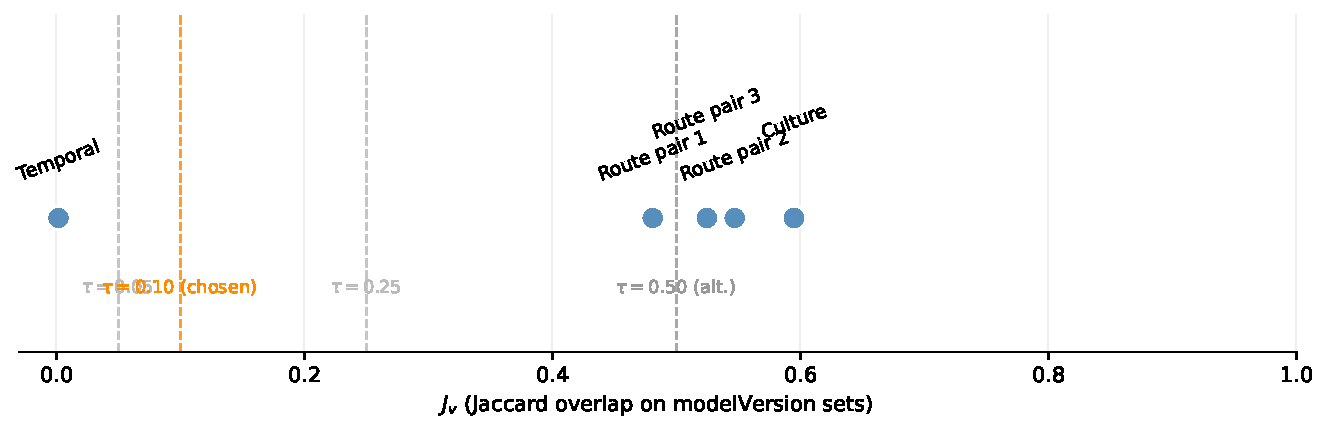
\includegraphics[width=0.95\linewidth]{tables/jaccard_threshold_sensitivity}
\caption{Observed $J_v$ values per L5B15 split, with candidate thresholds $\tau$ marked. The strongly bimodal distribution (temporal near $0$, route and culture splits near $0.5$) places the chosen $\tau=0.10$ in an empty band where classifications are invariant.}
\label{fig:jaccard_sensitivity}
\end{figure}

\section{Decision Tree Bootstrap Reproducibility} \label{app:bootstrap_dt}

Table~\ref{tab:bootstrap_dt} reports within-sample DT reproducibility alongside the observed between-split Spearman rank correlation, for each L5B15 split. For each sub-sample the decision tree was re-fitted ten times with different random seeds, yielding 45 pairwise $\rho$ values per sub-sample; the within mean reported is the average across the two sub-samples involved in each split. The gap between within and between $\rho_{\text{DT}}$ separates instability attributable to genuine subgroup composition from random fitting noise. Three of the five splits show gaps above 0.10, classified as genuine signal. The NCE$\to$ORY vs TLS$\to$ORY split shows a negative gap, indicating that the between-split drop falls within the noise floor for that particular route pair.

\begin{table}
\caption{Within-sample DT reproducibility versus observed between-split $\rho_S^{\mathrm{DT}}$. For each sub-sample the DT surrogate was re-fitted on identical data with $N=10$ random seeds, yielding 45 pairwise Spearman~$\rho$ values per sub-sample. Within (mean) is the average of those means across the two sub-samples of each split. Gap $=$ Within $-$ Between. Classification: $>0.10$ genuine signal; $0.03$ to $0.10$ small effect; $\leq 0.03$ indistinguishable from refit noise.}
\label{tab:bootstrap_dt}
\begin{tabular}{lrrrl}
\toprule
Split & Within (mean) & Between & Gap & Classification \\
\midrule
ORY$\to$NCE vs ORY$\to$OPO & 0.824 & 0.510 & +0.314 & Genuine signal \\
ORY$\to$OPO vs NCE$\to$ORY & 0.789 & 0.584 & +0.206 & Genuine signal \\
NCE$\to$ORY vs TLS$\to$ORY & 0.802 & 0.817 & -0.015 & Within noise floor \\
Temporal (early vs late) & 0.935 & 0.855 & +0.080 & Small effect \\
Culture (fr-FR vs nl-NL) & 0.977 & 0.666 & +0.310 & Genuine signal \\
Routes (aggregate) & 0.813 & 0.637 & +0.176 & Genuine signal \\
\bottomrule
\end{tabular}
\end{table}


\section{Per-Split Top-10 Feature Rankings} \label{app:top10_per_split}

Table~\ref{tab:top10_l5b15_per_split} lists the ten highest-ranked features per L5B15 split per explanation method, taken directly from the saved per-split rankings used in the stability analysis. The qualitative agreement between SHAP and LIME on the top features, and the broader disagreement of the Decision Tree with both, mirrors the quantitative pattern reported in the stability matrix (Table~\ref{tab:stability_l5b15}).

\begin{table}
\caption{Top-10 feature attributions per L5B15 split per explanation method.}
\label{tab:top10_l5b15_per_split}
\begin{tabular}{l p{4.2cm} p{4.2cm} p{4.2cm}}
\toprule
split & DT & SHAP & LIME \\
\midrule
early & 1. Email.Out.Pending.HistCount \newline 2. Param.BundleName \newline 3. Email.Out.Delivered.LastOut.Days \newline 4. Email.In.Clicked.LastOut.Days \newline 5. Push.Out.Pending.LastOut.Days \newline 6. FlightInboundArrival \newline 7. Email.Out.Pending.LastOut.Days \newline 8. SeatNumber \newline 9. Email.In.Pending.LastOut.Days \newline 10. Journey & 1. Param.BundleName \newline 2. Email.Out.Pending.LastOut.Days \newline 3. Push.Out.Pending.LastGroup \newline 4. Email.Out.Delivered.LastOut.Days \newline 5. SeatNumber \newline 6. IsStaffStandBy \newline 7. BookingMonth \newline 8. Email.Out.Pending.LastGroup \newline 9. Email.Out.Pending.HistCount \newline 10. FlightInboundArrival & 1. Param.BundleName \newline 2. SeatNumber \newline 3. IsStaffStandBy \newline 4. BookingMonth \newline 5. Email.Out.Pending.LastOut.Days \newline 6. Email.Out.Pending.HistCount \newline 7. Email.In.Clicked.LastOut.Days \newline 8. Email.Out.Delivered.LastOut.Days \newline 9. DestinationAirport \newline 10. Language \\
late & 1. Email.Out.Pending.HistCount \newline 2. Email.In.Clicked.LastOut.Days \newline 3. Param.BundleName \newline 4. Push.Out.Pending.HistCount \newline 5. Email.Out.Delivered.LastOut.Days \newline 6. Email.In.Pending.LastOut.Days \newline 7. SeatNumber \newline 8. Email.Out.Pending.LastOut.Days \newline 9. BookingMonth \newline 10. FlightInboundArrival & 1. Param.BundleName \newline 2. Email.Out.Pending.LastOut.Days \newline 3. Push.Out.Pending.LastGroup \newline 4. Email.Out.Delivered.LastOut.Days \newline 5. SeatNumber \newline 6. Email.Out.Pending.LastGroup \newline 7. BookingMonth \newline 8. IsStaffStandBy \newline 9. Email.Out.Pending.HistCount \newline 10. FlightInboundArrival & 1. Param.BundleName \newline 2. SeatNumber \newline 3. IsStaffStandBy \newline 4. BookingMonth \newline 5. Email.Out.Pending.LastOut.Days \newline 6. Email.Out.Pending.HistCount \newline 7. DestinationAirport \newline 8. Email.In.Clicked.LastOut.Days \newline 9. Email.Out.Delivered.LastOut.Days \newline 10. FlightInboundArrival \\
ORY$\to$NCE & 1. Email.Out.Delivered.LastOut.Days \newline 2. Param.BundleName \newline 3. Push.Out.Pending.HistCount \newline 4. Email.Out.Pending.LastOut.Days \newline 5. Email.In.Clicked.LastOut.Days \newline 6. FlightInboundArrival \newline 7. BookingMonth \newline 8. IH.Event.Outbound.RealTimeEvent.HistCount \newline 9. Journey \newline 10. Push.Out.Pending.LastGroup & 1. Param.BundleName \newline 2. Email.Out.Pending.LastOut.Days \newline 3. Push.Out.Pending.LastGroup \newline 4. SeatNumber \newline 5. Email.Out.Delivered.LastOut.Days \newline 6. Email.Out.Pending.LastGroup \newline 7. IsStaffStandBy \newline 8. Email.Out.Pending.HistCount \newline 9. BookingMonth \newline 10. FlightInboundArrival & 1. Param.BundleName \newline 2. SeatNumber \newline 3. IsStaffStandBy \newline 4. BookingMonth \newline 5. DestinationAirport \newline 6. Email.Out.Pending.LastOut.Days \newline 7. Email.Out.Pending.HistCount \newline 8. Email.In.Clicked.LastOut.Days \newline 9. Email.Out.Delivered.LastOut.Days \newline 10. Email.Out.Pending.LastGroup \\
ORY$\to$OPO & 1. Email.Out.Pending.LastOut.Days \newline 2. Param.BundleName \newline 3. Email.In.Pending.LastOut.Days \newline 4. Email.Out.Delivered.LastOut.Days \newline 5. DestinationAirport \newline 6. CultureCode \newline 7. FlightInboundArrival \newline 8. Language \newline 9. Journey \newline 10. FlightNumberOperatorIATA & 1. Param.BundleName \newline 2. Email.Out.Pending.LastOut.Days \newline 3. Push.Out.Pending.LastGroup \newline 4. Email.Out.Delivered.LastOut.Days \newline 5. SeatNumber \newline 6. IsStaffStandBy \newline 7. Email.Out.Pending.LastGroup \newline 8. Email.Out.Pending.HistCount \newline 9. BookingMonth \newline 10. FlightInboundArrival & 1. Param.BundleName \newline 2. SeatNumber \newline 3. IsStaffStandBy \newline 4. BookingMonth \newline 5. Email.Out.Pending.LastOut.Days \newline 6. DestinationAirport \newline 7. Email.Out.Pending.HistCount \newline 8. Email.Out.Delivered.LastOut.Days \newline 9. Language \newline 10. Email.In.Clicked.LastOut.Days \\
NCE$\to$ORY & 1. Email.Out.Pending.HistCount \newline 2. Param.BundleName \newline 3. Email.Out.Delivered.LastOut.Days \newline 4. Push.Out.Pending.LastOut.Days \newline 5. BookerGender \newline 6. Email.Out.Pending.LastOut.Days \newline 7. BookingMonth \newline 8. Email.In.Pending.LastOut.Days \newline 9. Journey \newline 10. IH.Event.Outbound.RealTimeEvent.HistCount & 1. Param.BundleName \newline 2. Email.Out.Pending.LastOut.Days \newline 3. Email.Out.Delivered.LastOut.Days \newline 4. Push.Out.Pending.LastGroup \newline 5. SeatNumber \newline 6. IsStaffStandBy \newline 7. Email.Out.Pending.LastGroup \newline 8. Email.Out.Pending.HistCount \newline 9. BookingMonth \newline 10. Language & 1. Param.BundleName \newline 2. SeatNumber \newline 3. IsStaffStandBy \newline 4. BookingMonth \newline 5. Email.Out.Pending.LastOut.Days \newline 6. Email.Out.Pending.HistCount \newline 7. Email.In.Clicked.LastOut.Days \newline 8. FlightInboundArrival \newline 9. Language \newline 10. Email.Out.Delivered.LastOut.Days \\
TLS$\to$ORY & 1. Email.Out.Pending.HistCount \newline 2. Param.BundleName \newline 3. Push.Out.Pending.LastOut.Days \newline 4. Email.Out.Delivered.LastOut.Days \newline 5. BookingMonth \newline 6. BookerGender \newline 7. Language \newline 8. Journey \newline 9. FlightNumberOperatorIATA \newline 10. SeatNumber & 1. Param.BundleName \newline 2. Email.Out.Pending.LastOut.Days \newline 3. IsStaffStandBy \newline 4. Push.Out.Pending.LastGroup \newline 5. Email.Out.Delivered.LastOut.Days \newline 6. SeatNumber \newline 7. Email.Out.Pending.LastGroup \newline 8. Email.Out.Pending.HistCount \newline 9. BookingMonth \newline 10. FlightInboundArrival & 1. Param.BundleName \newline 2. SeatNumber \newline 3. IsStaffStandBy \newline 4. BookingMonth \newline 5. Email.Out.Pending.LastOut.Days \newline 6. Email.Out.Pending.HistCount \newline 7. Language \newline 8. FlightInboundArrival \newline 9. Email.In.Clicked.LastOut.Days \newline 10. Email.Out.Delivered.LastOut.Days \\
fr-FR & 1. Email.Out.Pending.HistCount \newline 2. Email.In.Clicked.LastOut.Days \newline 3. Param.BundleName \newline 4. IsStaffStandBy \newline 5. Email.Out.Delivered.LastOut.Days \newline 6. Email.Out.Pending.LastOut.Days \newline 7. SeatNumber \newline 8. Push.Out.Pending.HistCount \newline 9. Push.Out.Pending.LastOut.Days \newline 10. Push.Out.Pending.LastGroup & 1. Param.BundleName \newline 2. Email.Out.Pending.LastOut.Days \newline 3. Push.Out.Pending.LastGroup \newline 4. Email.Out.Delivered.LastOut.Days \newline 5. SeatNumber \newline 6. Email.Out.Pending.LastGroup \newline 7. IsStaffStandBy \newline 8. Email.Out.Pending.HistCount \newline 9. BookingMonth \newline 10. FlightInboundArrival & 1. Param.BundleName \newline 2. SeatNumber \newline 3. IsStaffStandBy \newline 4. BookingMonth \newline 5. Email.Out.Pending.LastOut.Days \newline 6. Email.Out.Pending.HistCount \newline 7. DestinationAirport \newline 8. Email.Out.Delivered.LastOut.Days \newline 9. Language \newline 10. Email.Out.Pending.LastGroup \\
nl-NL & 1. Param.BundleName \newline 2. Email.Out.Pending.LastOut.Days \newline 3. Email.Out.Delivered.LastOut.Days \newline 4. Email.Out.Pending.HistCount \newline 5. Push.Out.Pending.LastOut.Days \newline 6. Push.Out.Pending.LastGroup \newline 7. FlightInboundArrival \newline 8. SeatNumber \newline 9. IsStaffStandBy \newline 10. IH.Event.Outbound.RealTimeEvent.HistCount & 1. Param.BundleName \newline 2. Push.Out.Pending.LastGroup \newline 3. Email.Out.Pending.LastOut.Days \newline 4. SeatNumber \newline 5. BookingMonth \newline 6. Email.Out.Delivered.LastOut.Days \newline 7. IsStaffStandBy \newline 8. Email.Out.Pending.HistCount \newline 9. FlightInboundArrival \newline 10. Email.Out.Pending.LastGroup & 1. Param.BundleName \newline 2. SeatNumber \newline 3. IsStaffStandBy \newline 4. BookingMonth \newline 5. Email.Out.Pending.LastOut.Days \newline 6. Email.Out.Pending.HistCount \newline 7. DestinationAirport \newline 8. Email.In.Clicked.LastOut.Days \newline 9. FlightInboundArrival \newline 10. Email.Out.Delivered.LastOut.Days \\
\bottomrule
\end{tabular}
\end{table}


\newpage

\chapter{Appendix on Generative Artificial Intelligence Use}

Generative AI was used throughout this thesis in the following ways.

\textbf{Research design and structuring.} Claude (Anthropic) was used to discuss and refine the research design, sharpen research questions, and structure the methodology chapter. AI-generated suggestions were critically evaluated and revised before incorporation.

\textbf{Writing and editing.} Claude was used to draft, restructure, and improve prose across all chapters. All AI-generated text was reviewed, adjusted, and rewritten where necessary to reflect the author's own reasoning and conclusions.

\textbf{Code assistance.} Claude and GitHub Copilot were used to assist with writing Python notebook cells for data ingestion, EDA, modelling, and visualisation. All code was reviewed, tested, and adapted by the author.

\textbf{LaTeX formatting.} Claude was used to generate and debug LaTeX code for tables, figures, and tikz diagrams.

\noindent Representative prompts used include:

\begin{itemize}
\item ``Critically evaluate my introduction draft and identify inconsistencies with the actual data constraints.''
\item ``How should I structure the methodology section for a thesis comparing XAI methods on a production propensity model?''
\item ``What does a problem formulation section in formal notation for a black-box surrogate explanation pipeline look like''
\item ``Generate a TikZ figure showing the full methodology pipeline from data to instability attribution.''
\end{itemize}

All final decisions regarding content, interpretation, and conclusions are the author's own. The use of generative AI did not affect the empirical analysis or the validity of the results.
\end{document}
